% Document template
\documentclass[a4paper,7pt]{article}

% Image packages
\usepackage{graphicx, pgf, tikz, pgfplots} 

\usepackage{fancyhdr}						% import fancy hdr
\usepackage{msdata}							% import mathscapes data
\usepackage{hyperref}
\usepackage[utf8]{inputenc}
\usepackage{siunitx}

% Set date
\usepackage{datetime}						% import datetime package
\newdate{date}{09}{09}{2019}				% set new date
\date{\displaydate{date}}					% configure doc date to new date

% Meta parameters
\setlength{\parindent}{0em}					% remove paragraph indent
\setlength{\parskip}{0.5em}					% set spacing after paragraph
\graphicspath{ {images/} }					% set images path
\fancyhf{}									% clear all header and footers
\renewcommand{\headrulewidth}{0pt}			% remove the header rule
\rfoot{\thepage}							% set page number in right footer
\pagestyle{fancy}							% set page styles as fancy
\lfoot{\mscpy}
\AtEndDocument{\lfoot{}}

% Copyright message
\chead{}

% Document Title
\title{Discoverdrome: Reimagining\\ Learning Spaces for 2101}
\author{ 
	Simran Singh \\
	\small{Mathscapes Research} \\
}

% Document
\begin{document}
\maketitle
\thispagestyle{fancy}

\begin{figure}[h]
  \center
  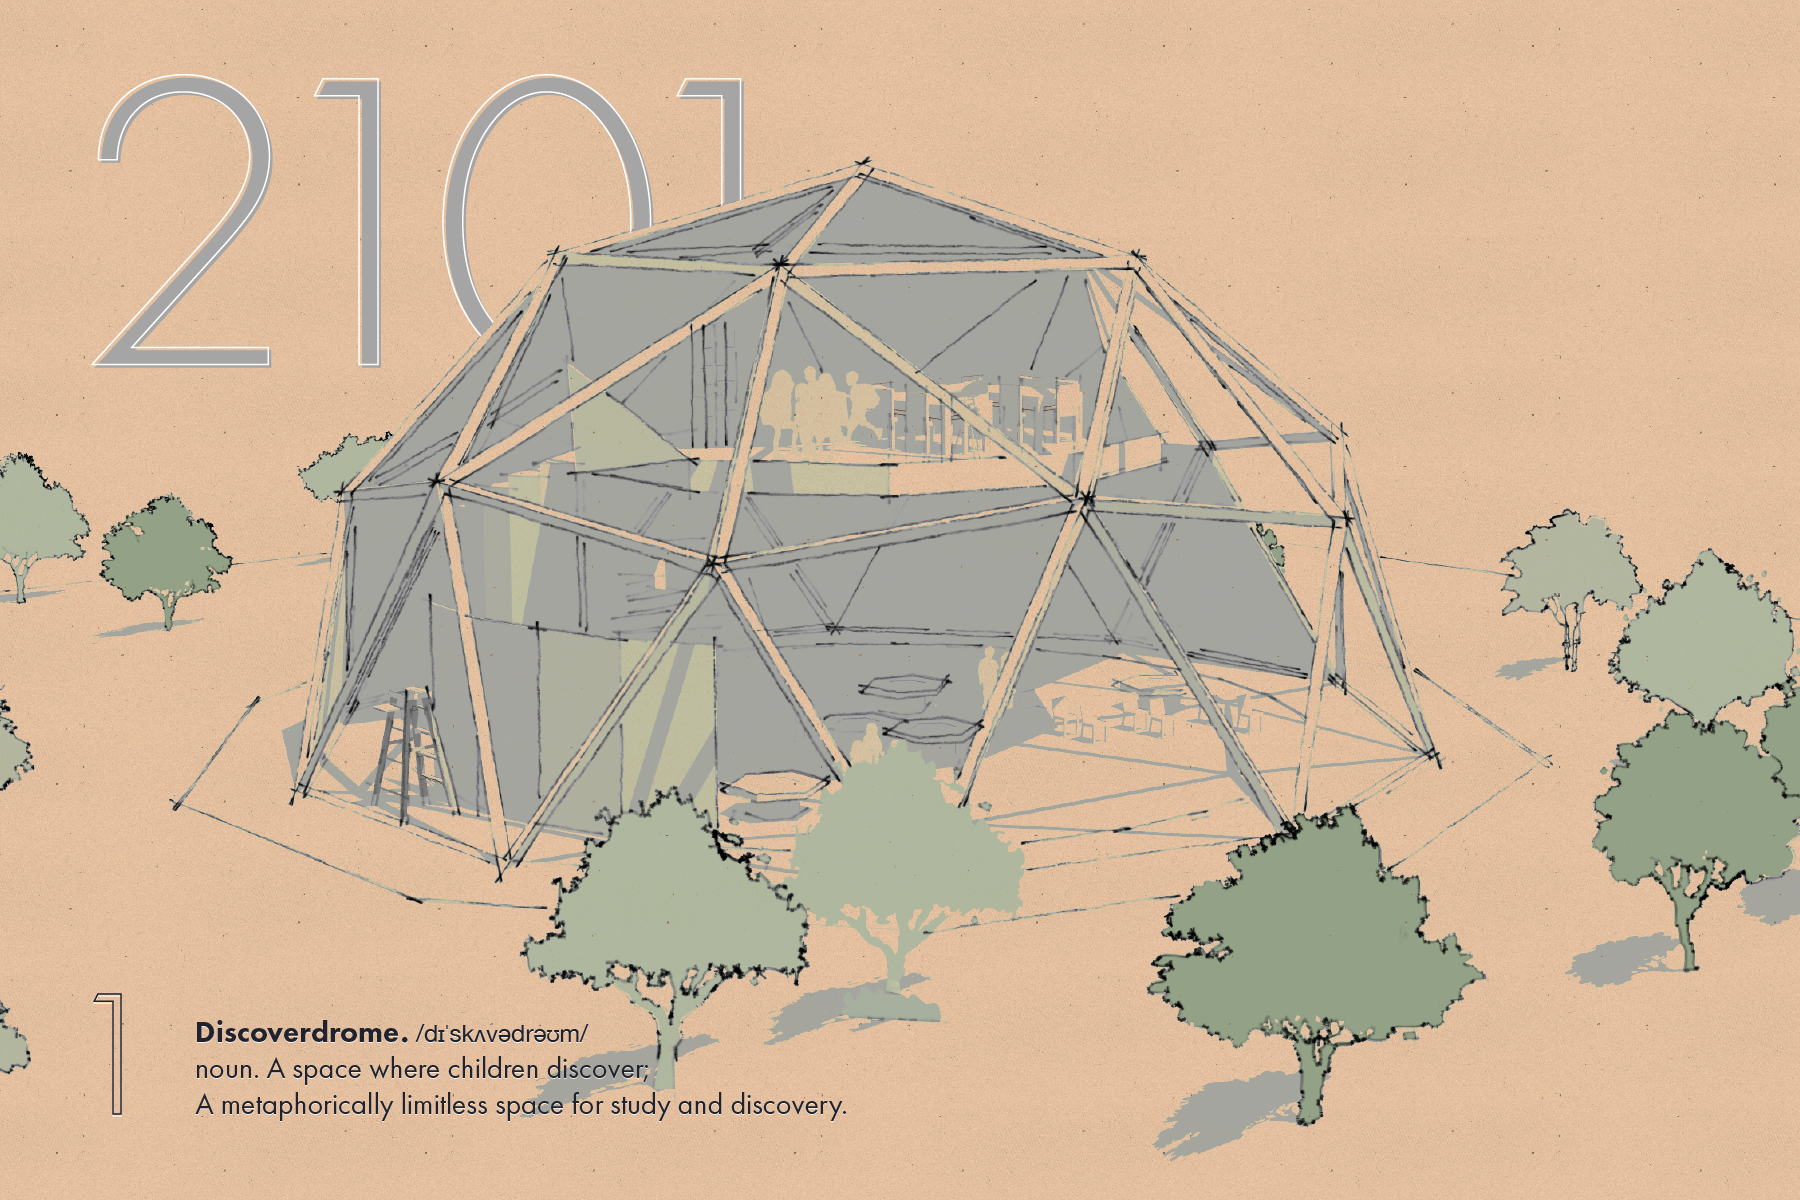
\includegraphics[width=\textwidth]{discoverdrome_1.png}
\end{figure}


\begin{abstract}
We wonder how the world will be by the end of this century. Would classrooms be the same as now, or will robots teach children? Does the tech-advancing world need humans to learn with/from machines, without learning about machines before? The needs of our present demand sustainable measures and conscious collaboration to best suit large-scale needs. This paper presents a note on a plausible design of such a learning space in 2101.
	
	\medskip
	\begin{center}
	\textit{Those who cannot remember the past are condemned to repeat it.}
	\\\footnotesize{-- George Santayana (From Vol. I, Reason in Common Sense in 1905)}
	\end{center}
\end{abstract}

\section{Introduction}
It is the year 2100 on the Earth, and a leading research institution is betting high on the future of education. Most technologies continue to obey Moore’s law and empower humans. Time machines exist discreetly in the multi-level security of \textit{Analemma}\footnote{Analemma is an upside down building, it is suspended from space and barely touches the Earth.}, a place beyond the Earth. The institution, expanding its scope of their research, extends several invites in the past to build a team of people from important times in history who would be assigned to design a Discoverdrome each that captures the best of ideas from their time.

\begin{quote}
	\textbf{Discoverdrome} \textit{noun.} A space where children discover; \\A metaphorically limitless space for study and discovery.
\end{quote}

\begin{figure}[h]
  \center
  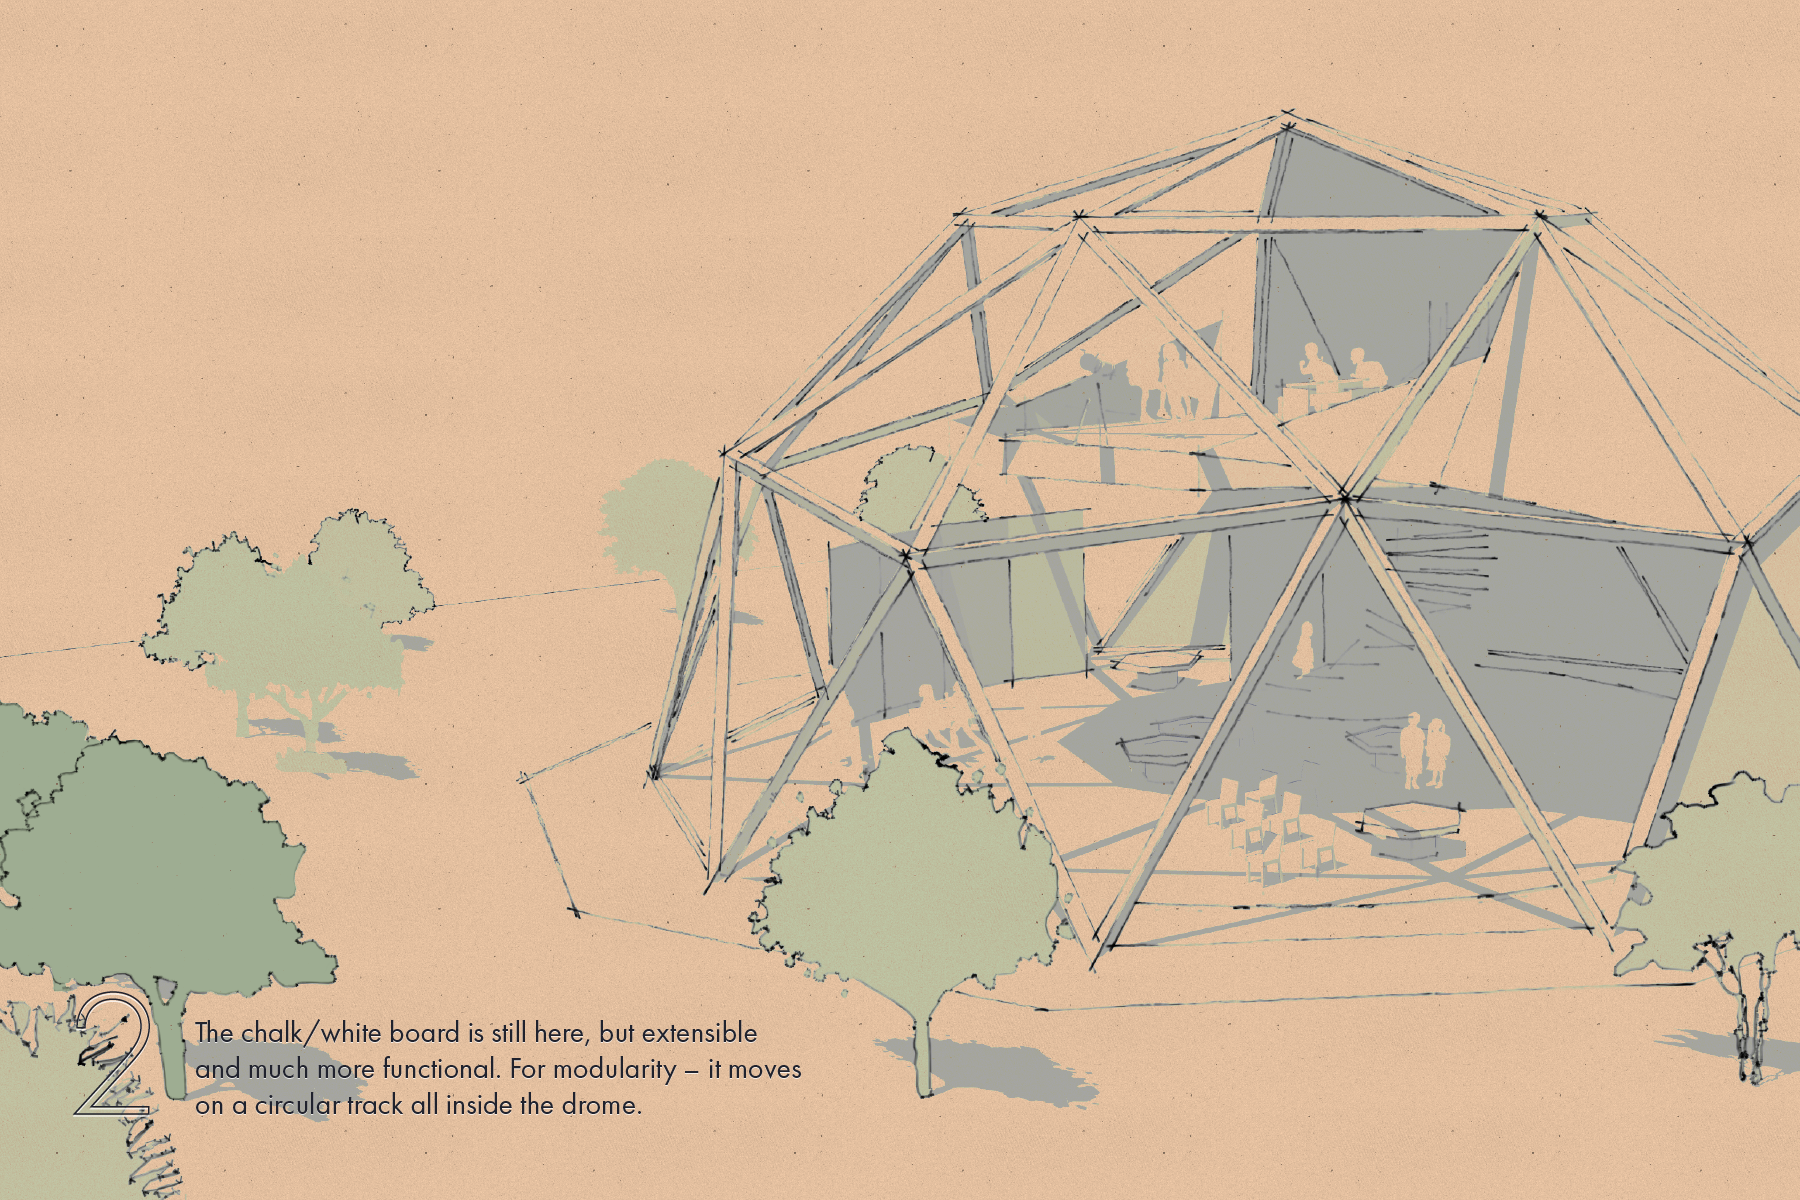
\includegraphics[width=0.9\textwidth]{discoverdrome_2.png}
\end{figure}

Motivated with this, I set out to explore if there is any sign of speculating a learning space in a distant future by any means. \textit{What will be my method of discussing and designing? Can research about present inform my decisions or if there is no point of the study?} But even with the remotest possibility of likelihood of this imagination transforming into reality sometime in the future, my research could help determine the suggested transition of our current needs and understanding for the educational demands for our upcoming future. Studying how the classrooms of our time shaped our own experiences, this exploration suggests the essentials as well as the expected we hope to impart to the future. 

In a future of its kind, the possibilities are bound to be complicated and ever-emerging. How then, the space for exploration for it be designed poorly? Believing that my perception for the future is accurate, the only real restrictions for the exploration were material and making. The study is steered by holding every little idea as a physical form in the Discoverdrome, disposable or reasonable to stay, further iterated or realized for the bigger picture. A sense of validation is gained by cross-checking whether ideologies are translated through every decision for space. Questions, not threatened by the factors of money and time are also raised through the process, giving value to experiences for a better design. The outcome of this exercise is a series of pictures describing the Discoverdrome, along with a letter to the one who finds it.

\begin{figure}[h]
  \center
  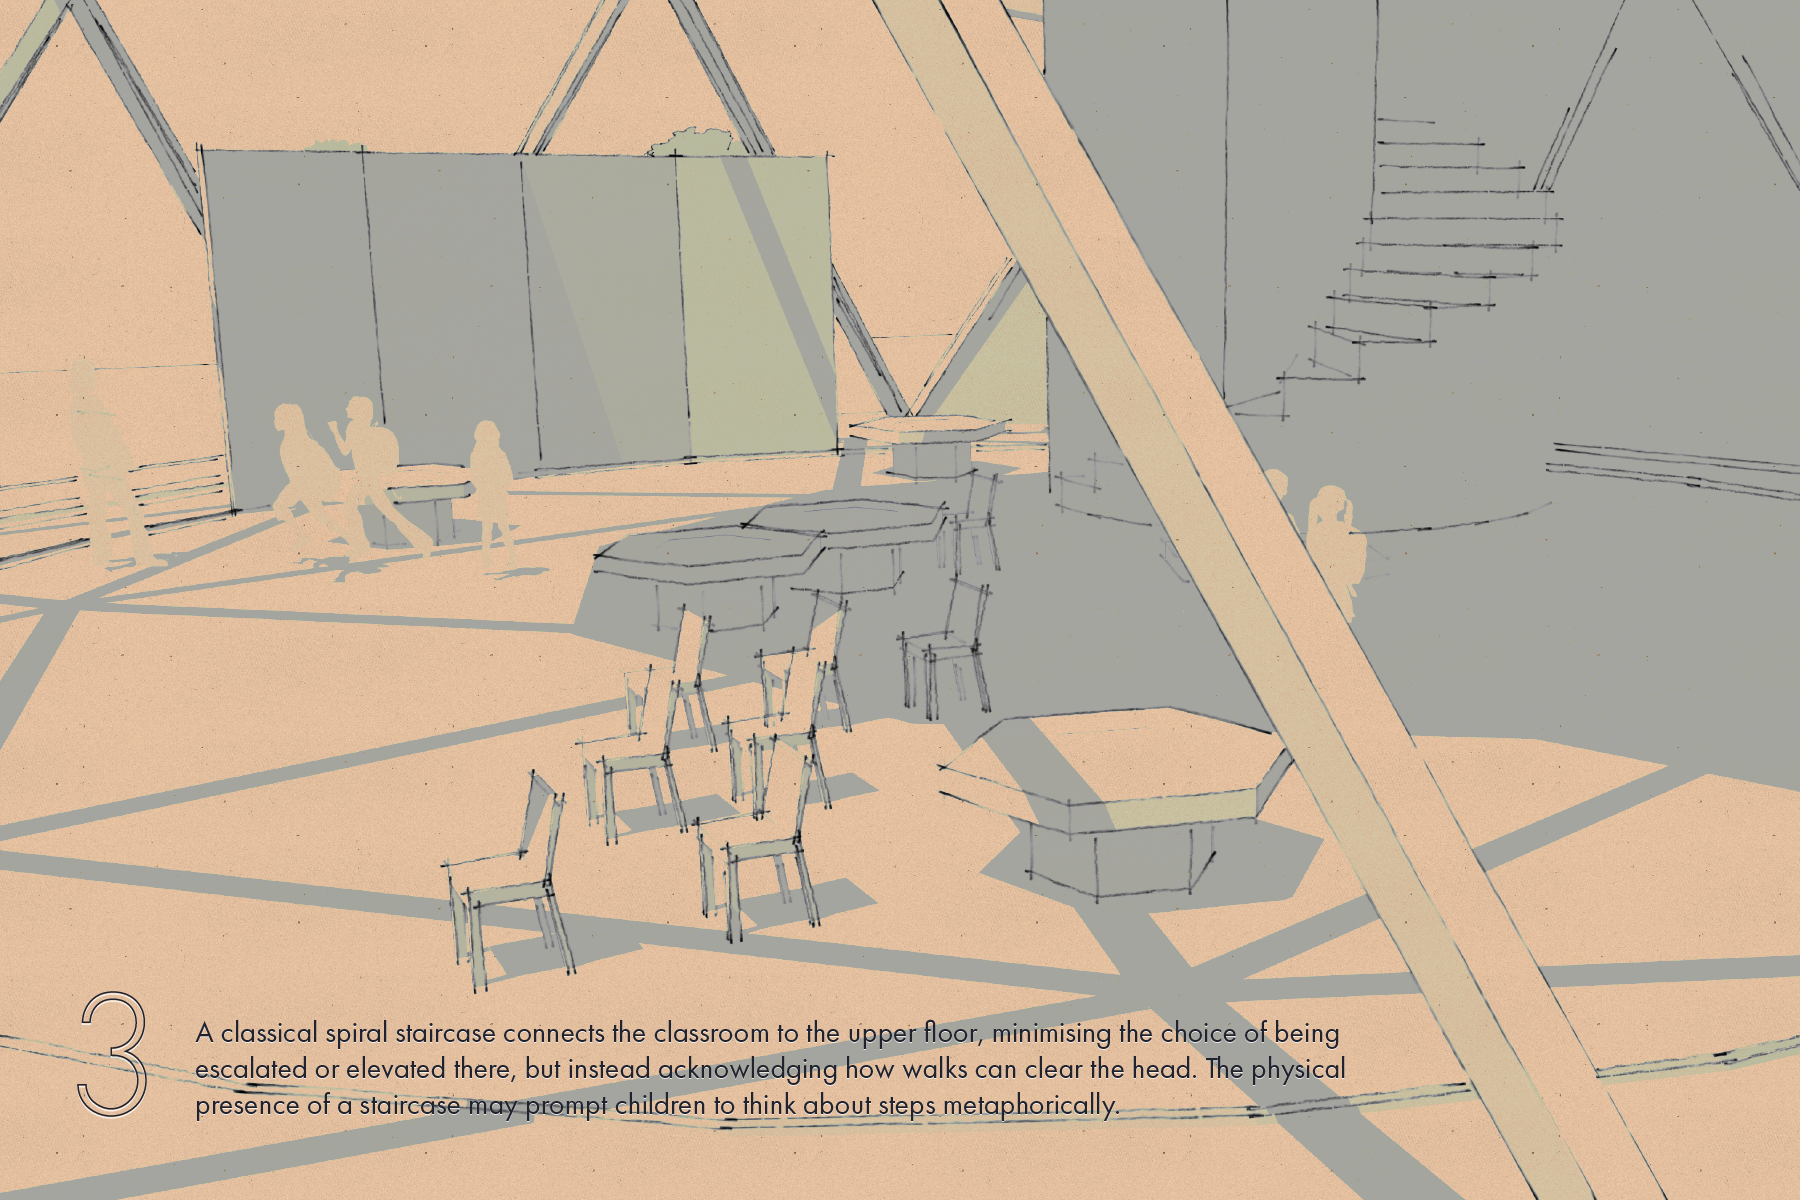
\includegraphics[width=0.9\textwidth]{discoverdrome_3.png}
\end{figure}

\section{Making}
Centering our approach towards collaborative learning and exploration in this space, it made sense, to begin with the ideal accommodation size in the classroom. Schools at our time had 25-50 children, sharing desks and learning from a regular, uniform timetable from a teacher, textbooks and a chalkboard. Our attention spans were delicate, and we see now how our ideal classroom should be more significant. The decided accommodation size was 12-18 people, with varied interests studying in the same space. The class would retain the board for teaching, as well as have room for advanced tools and techniques. This was decided to keep in mind that the experience of learning from a teacher in a classroom has a growing sense of curiosity throughout the process. Humans, as humans would continue to be unpredictable, compared to the omnipresence of machines, thus making teachers a crucial playmate in the learning process. Values such as respecting people and knowledge are also felt in such a setting. Space was given attributes such as: friendly, explorative, organized, and modular.

\begin{figure}[h]
  \center
  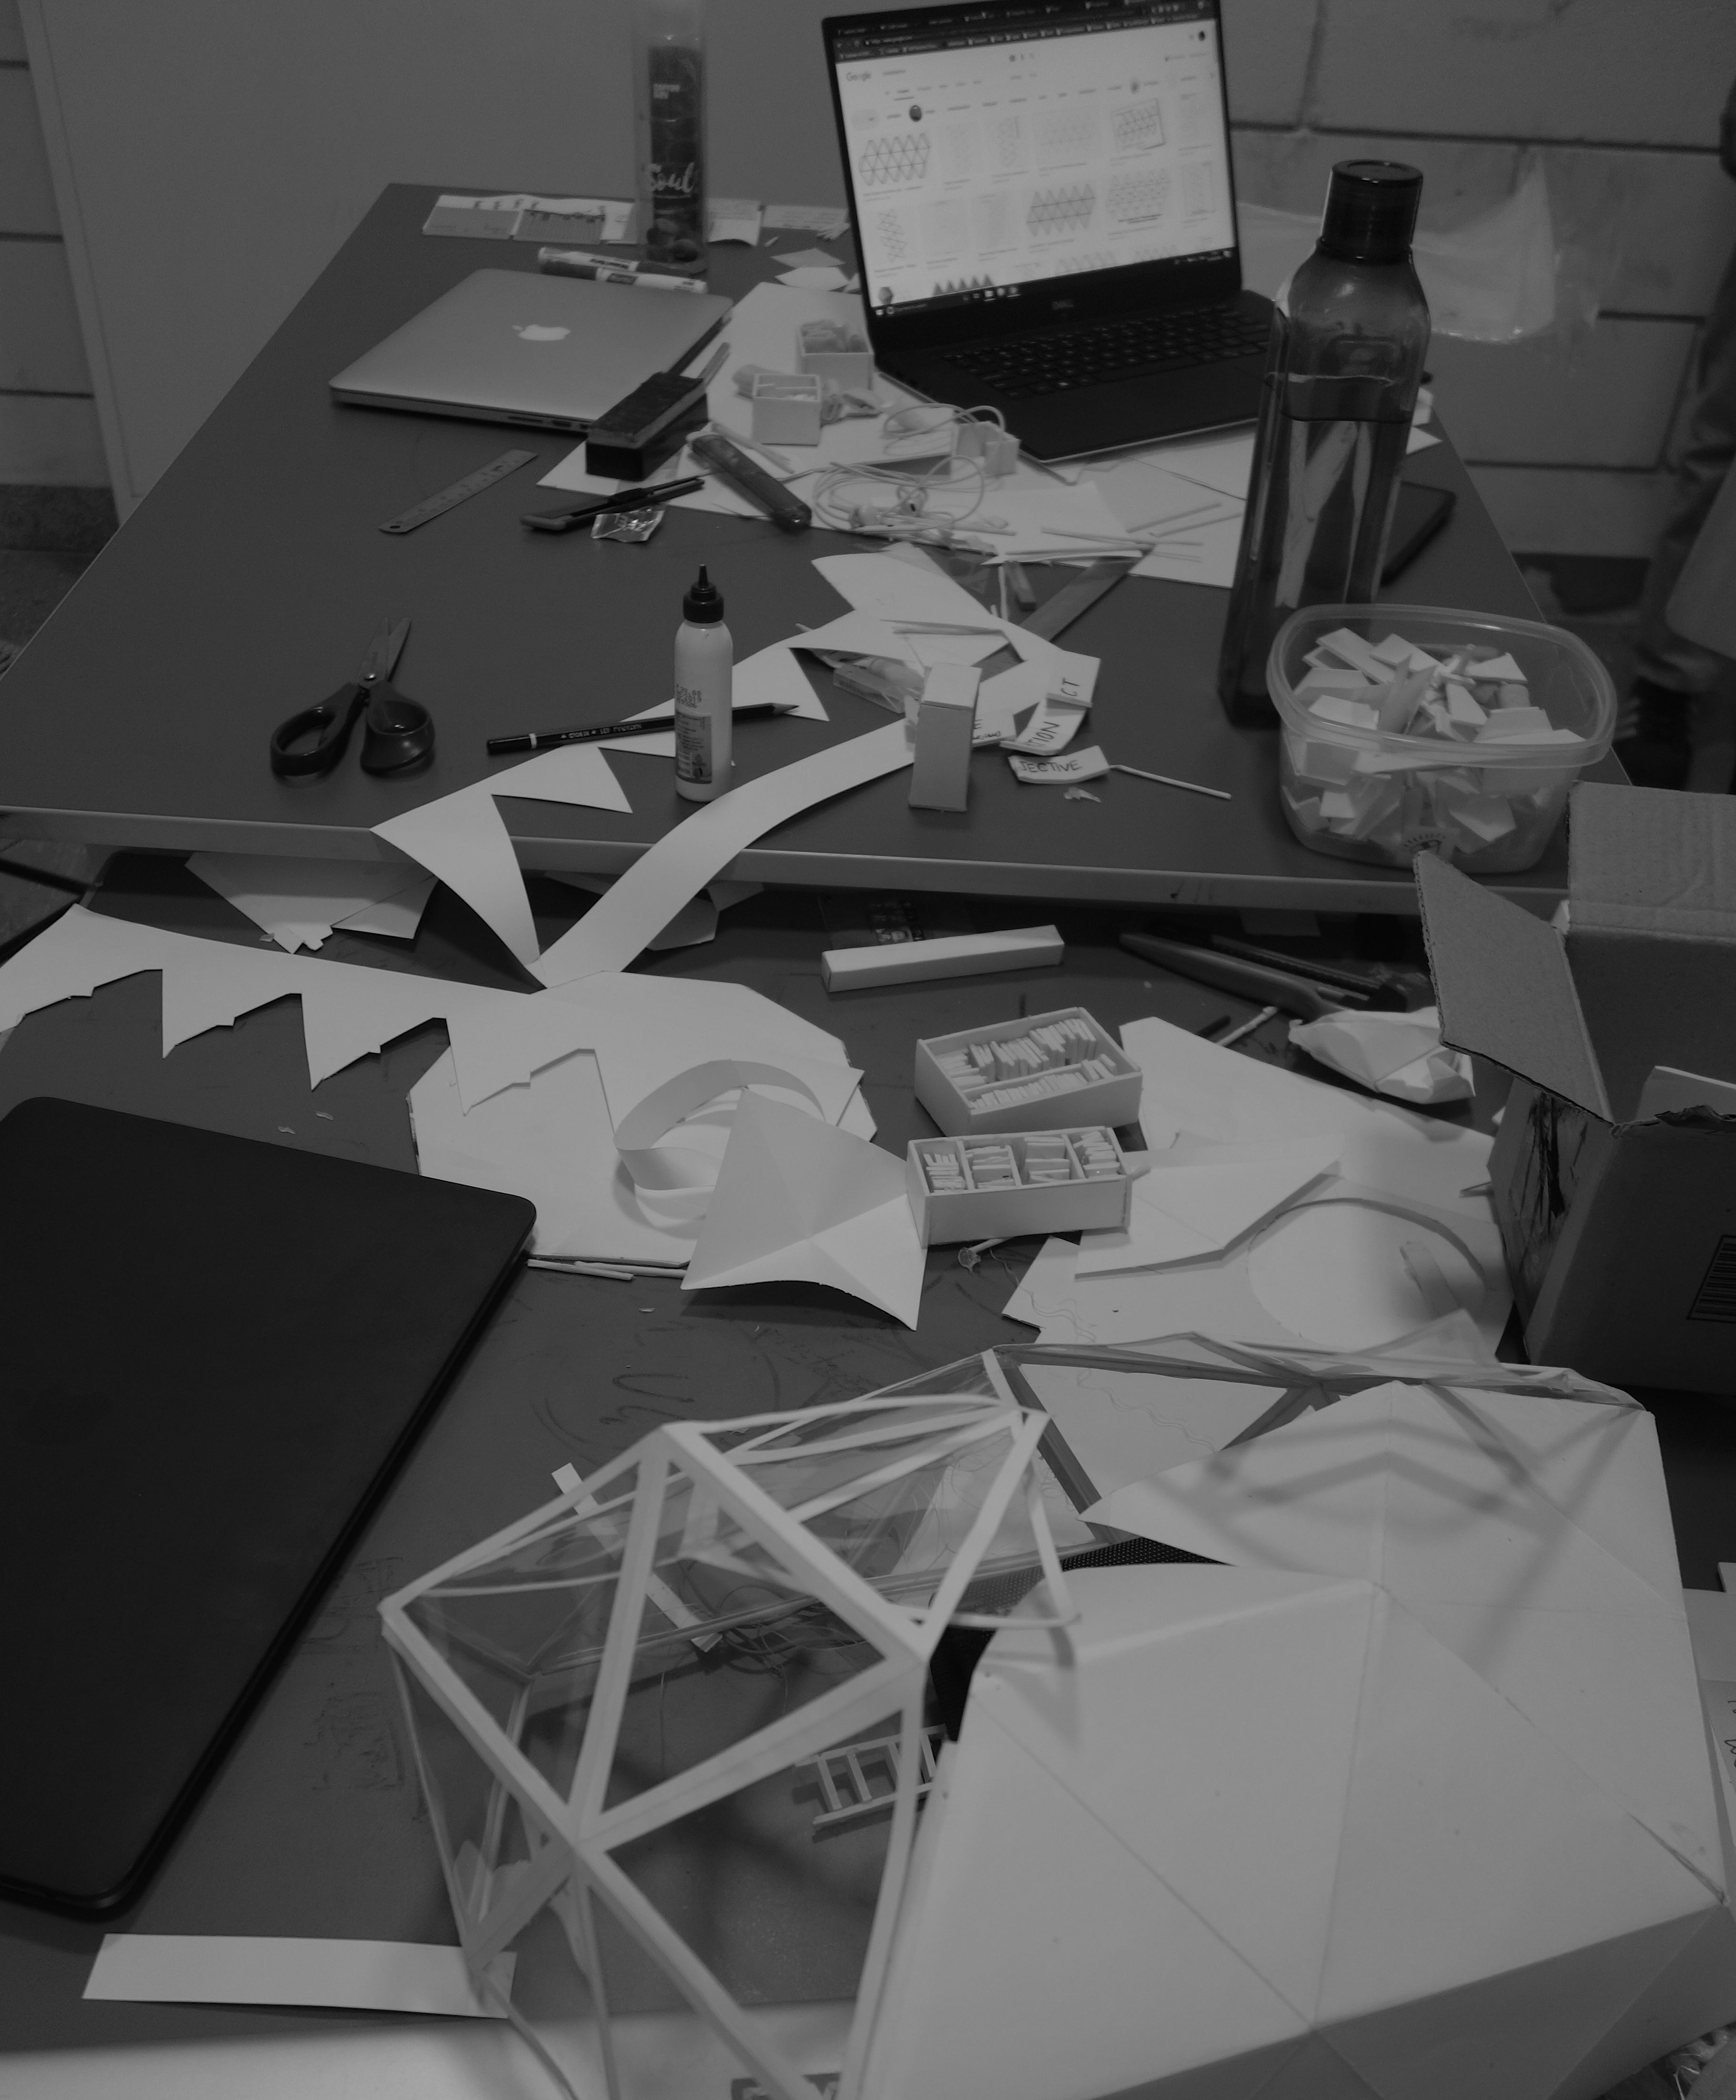
\includegraphics[width=0.3\textwidth]{making.jpg}
  \caption{Making of the geodesic dome took several attempts to perfect the desired icosahedron.}
\end{figure}

\subsection{Space}
Realizing that our classrooms were rigid and communal, I decide that the future should also provide room for personal space and exploration. It would perhaps be nice to have many corners in the place for children to occupy. An octagonal floor-plan was first laid out. 

\begin{figure}[h]
  \center
  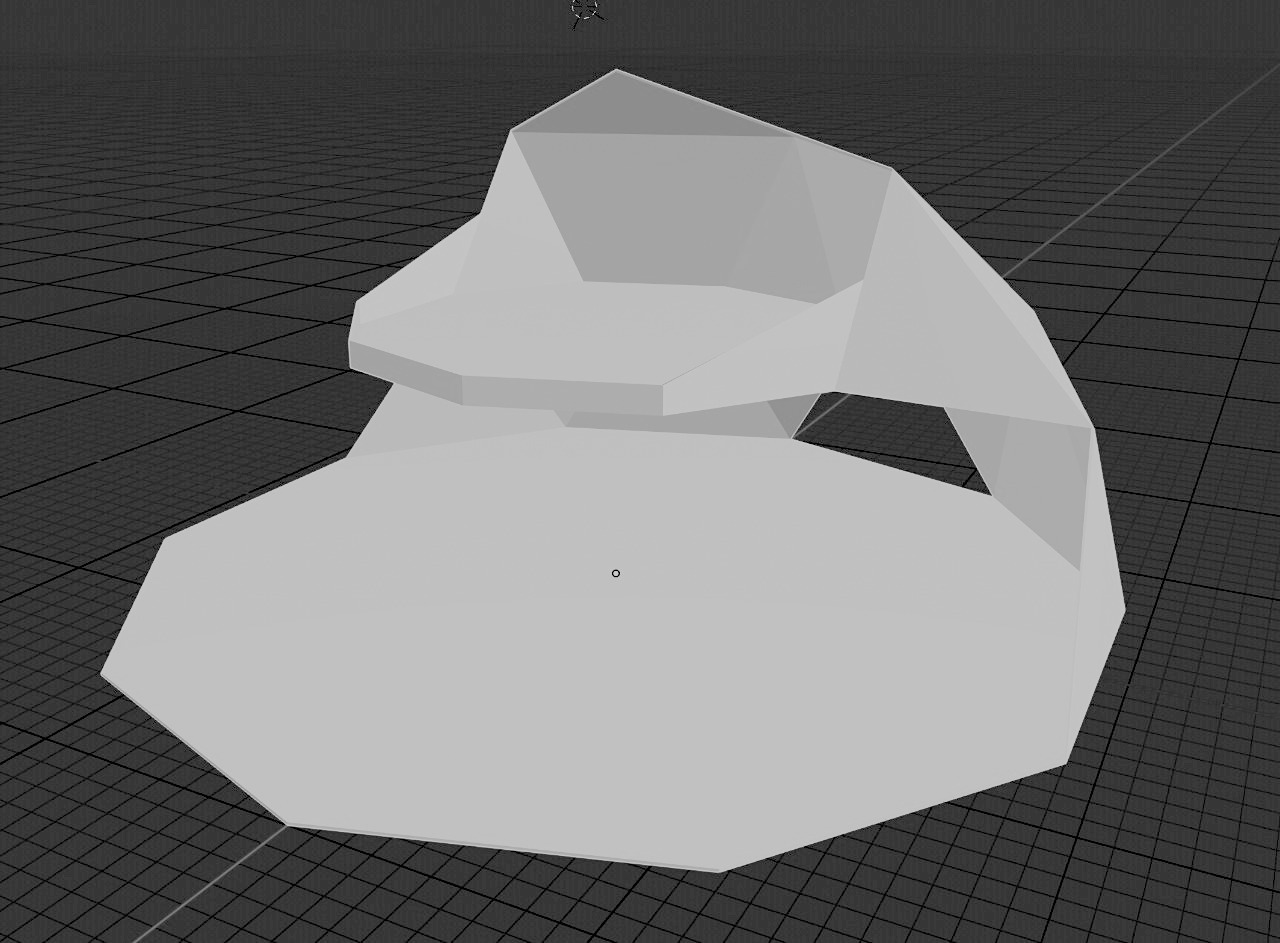
\includegraphics[height=0.15\textwidth]{dome1.jpg}
  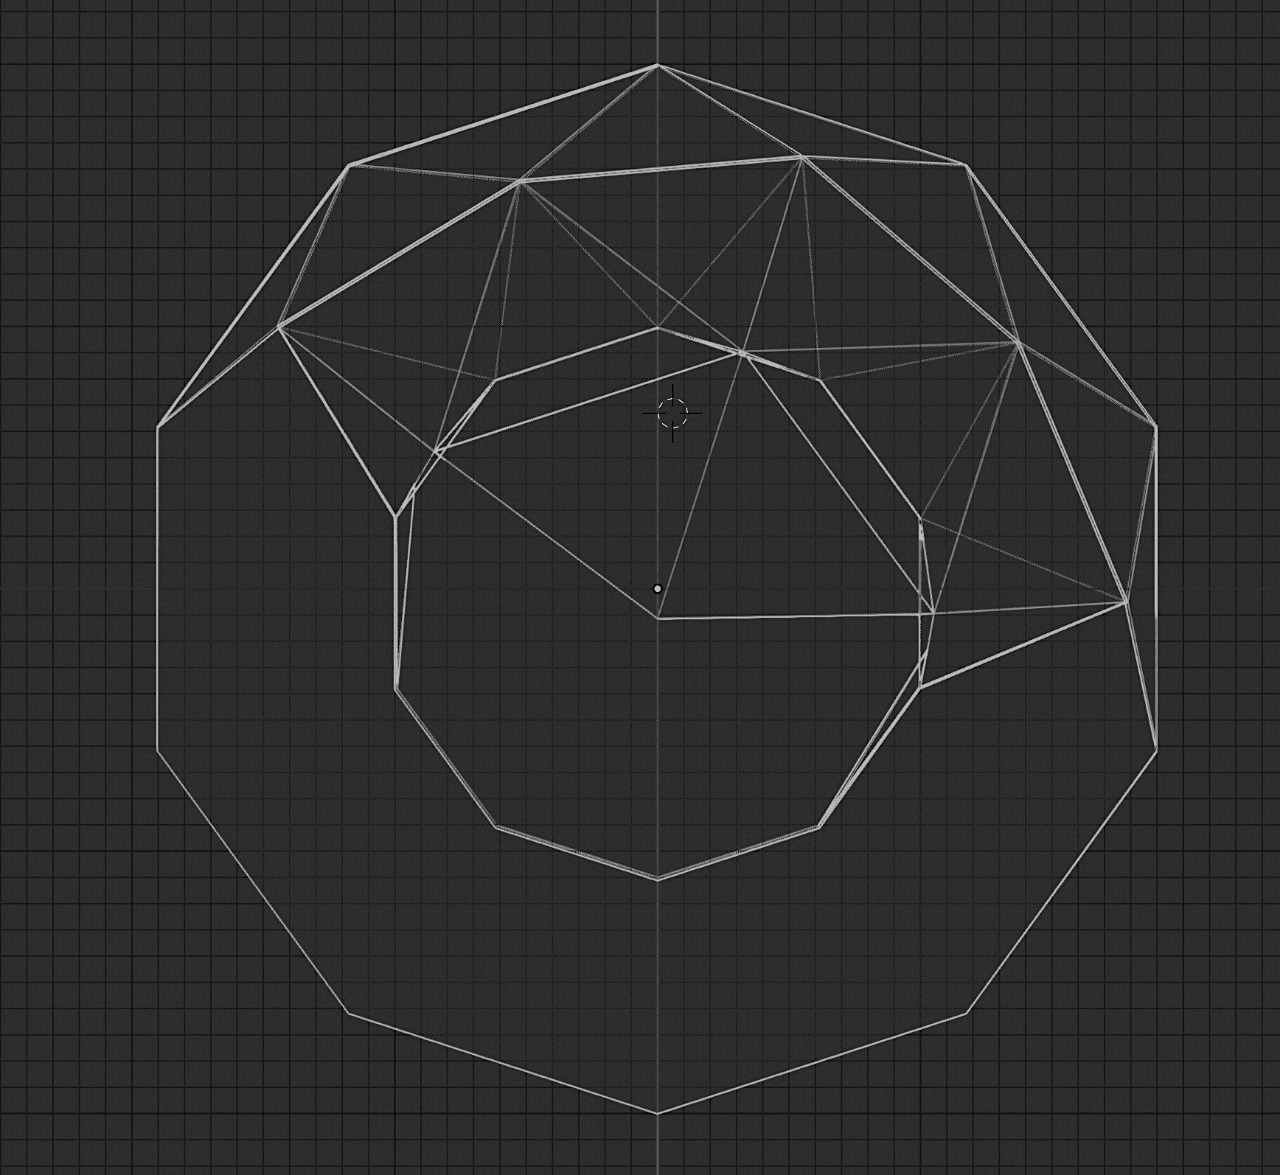
\includegraphics[height=0.15\textwidth]{dome2.jpg}
  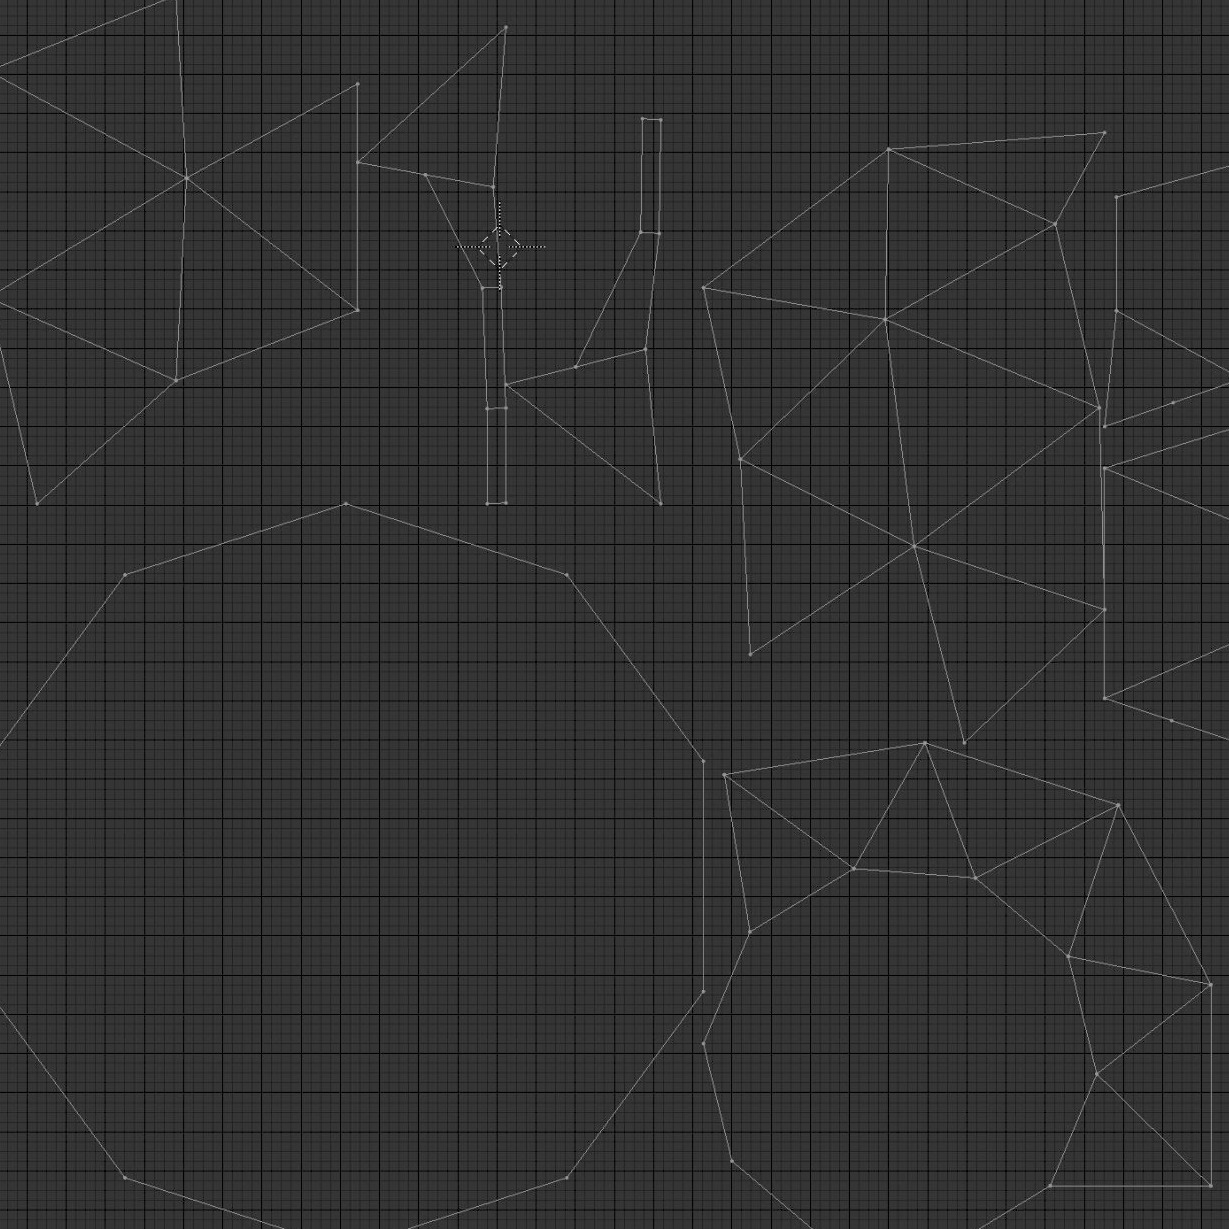
\includegraphics[height=0.15\textwidth]{dome3.jpg}
  \caption{3d renders of the dome skeleton}
\end{figure}

The scaling of objects concerning the laid out floor had us question whether eight sides are ideal when entrances could likely occupy two or more. We extended this exploration to Blender\footnote{Blender is a free and open-source 3D computer graphics software toolset.}, where the overall space was designed, keeping in mind- natural light and enough space. A library, like a to-go space within the classroom, was planned. It would be a floor above for proximity and a good view, smaller than the ground floor but acting as a balcony. This was also necessitated by fictional inspirations, where libraries often fancy knowledge as power. In my school once a week, I would have an hour-long library period. Other days, I would have to find the time and seek permissions to get time there during school hours. This hassle was not necessary. At Discoverdrome, anybody is open to visiting the library during their free time. Each classroom would have a unique collection of books, facilitated by machines for new demands. 

The approach to the library, upon discussion resonated with keeping things simple. A staircase acknowledges how also walks clear the head, placed near the entry door. Different forms were explored for the same.

\begin{figure}[h]
  \center
  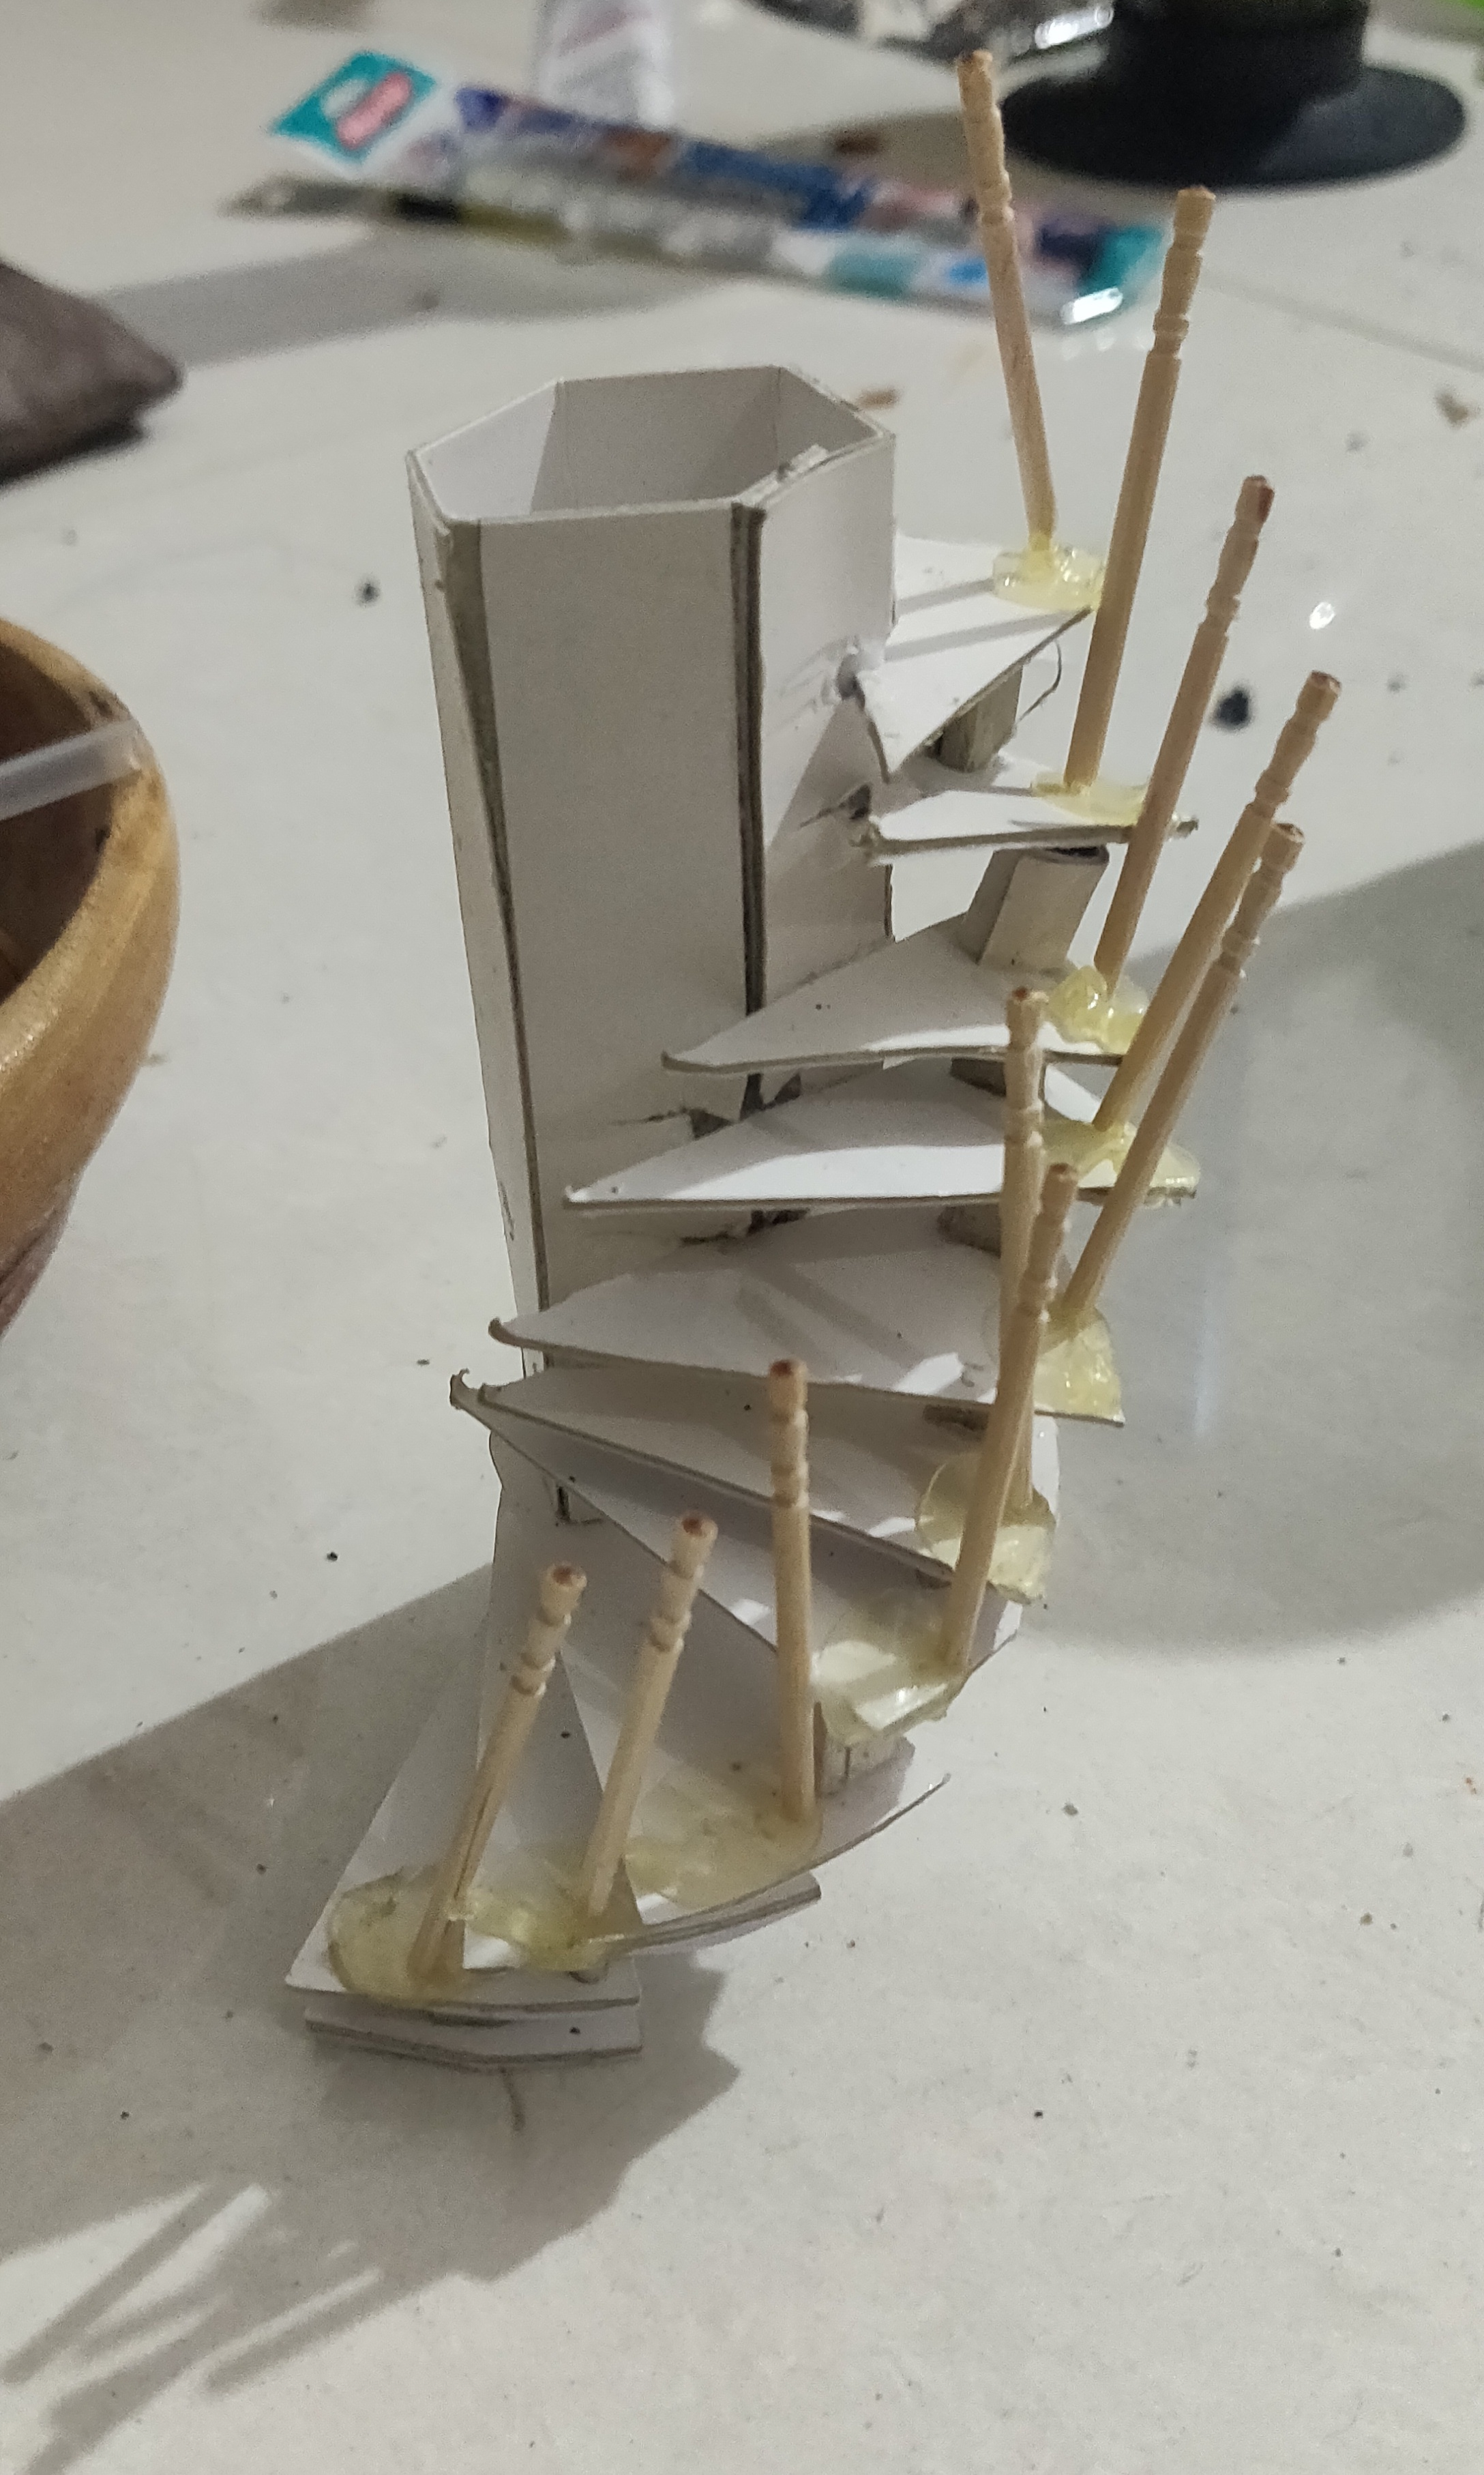
\includegraphics[height=0.2\textwidth]{steps0.jpg}
  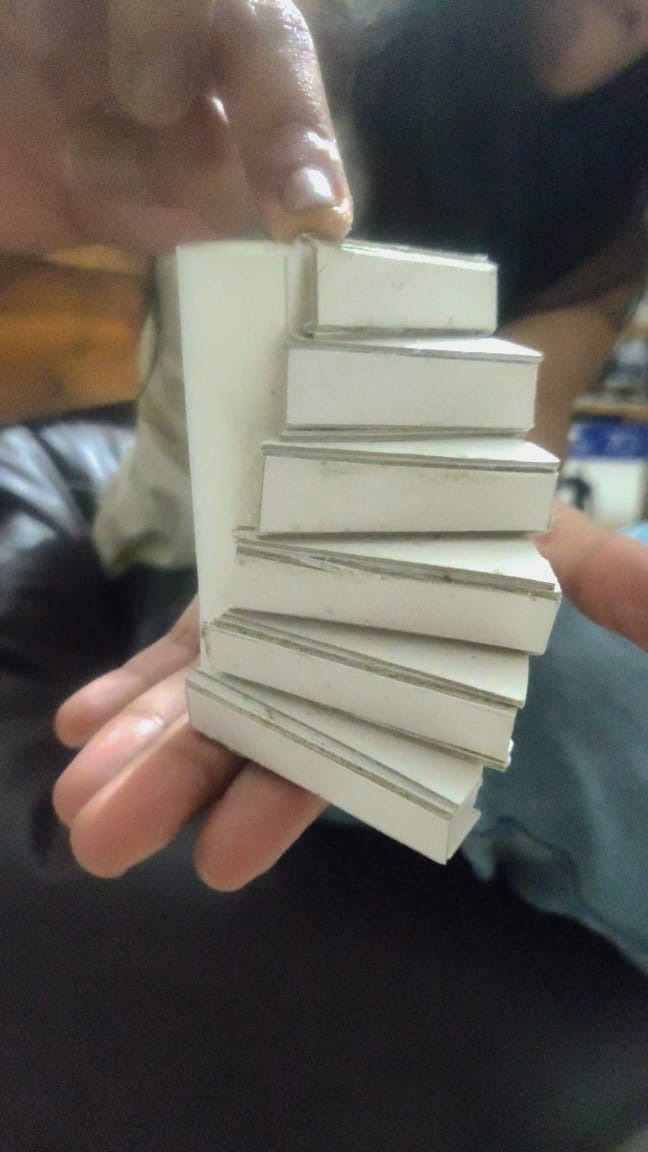
\includegraphics[height=0.2\textwidth]{steps1.jpg}
  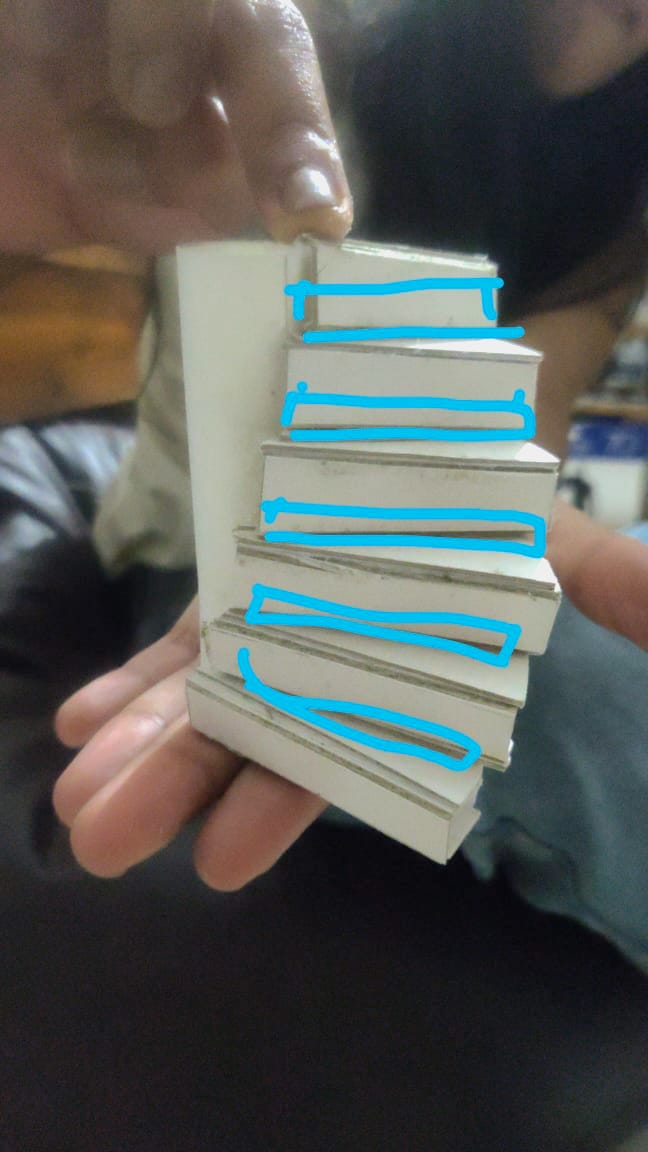
\includegraphics[height=0.2\textwidth]{steps2.jpg}
  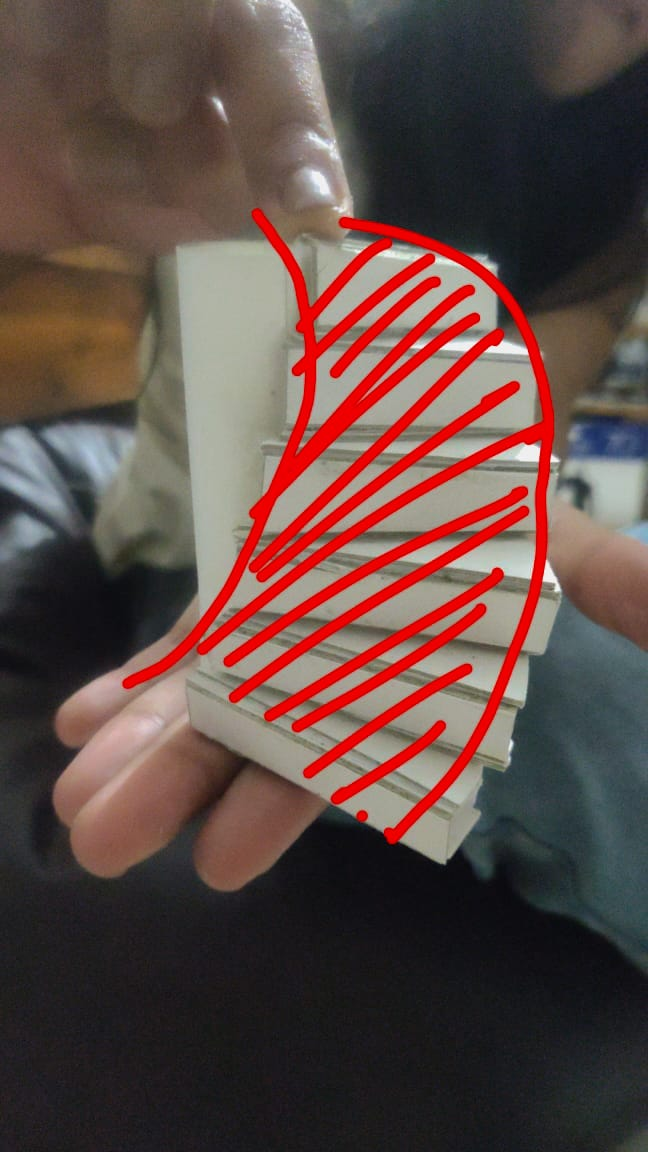
\includegraphics[height=0.2\textwidth]{steps3.jpg}
  \caption{Imagining spiral staircases with paper}
\end{figure}

There was a lack of uniformity because of material handling when it came to constructing the staircase. A circle with arcs from the center was used for the final steps. 

\begin{figure}[h]
  \center
  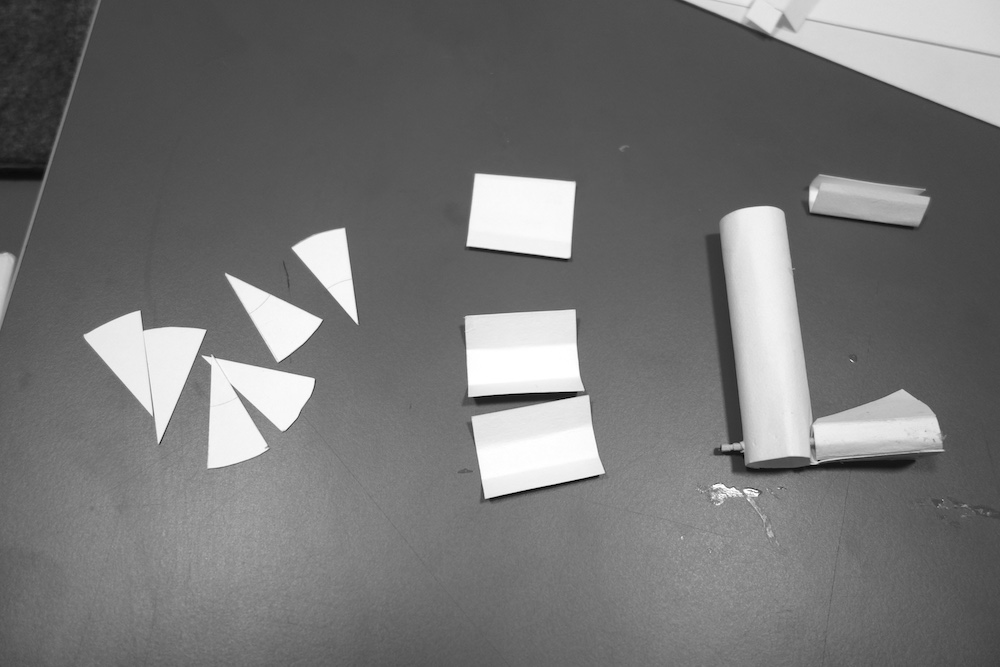
\includegraphics[height=0.13\textwidth]{steps4.jpg}
  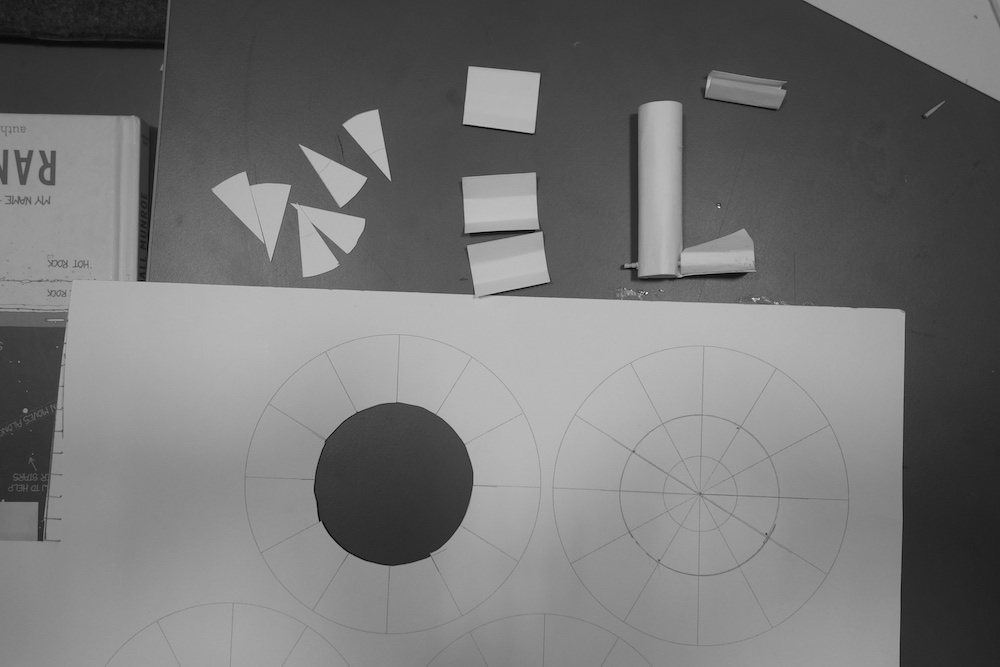
\includegraphics[height=0.13\textwidth]{steps5.jpg}
  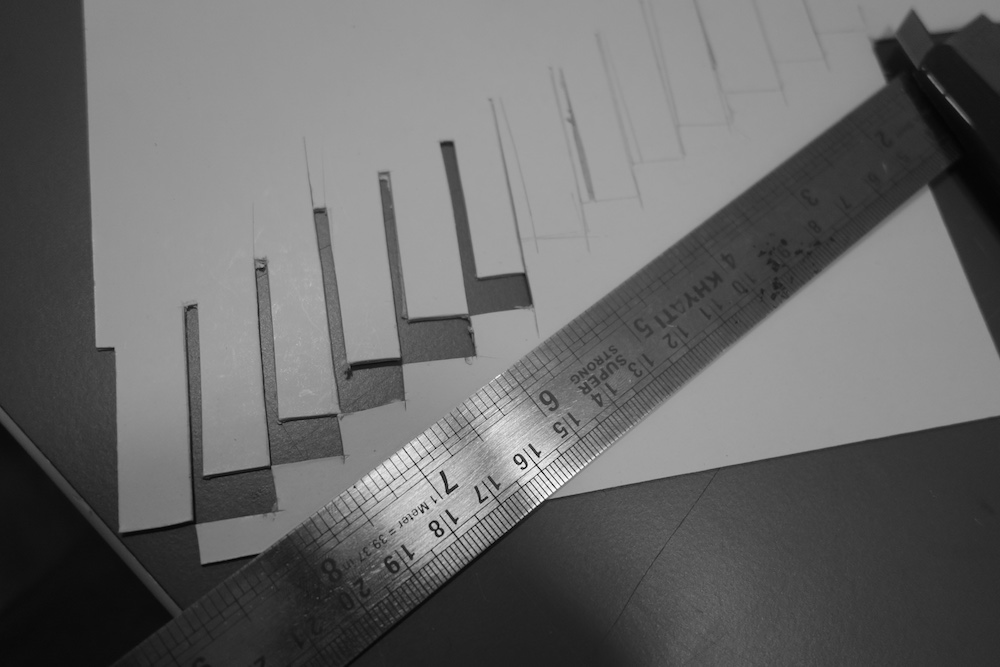
\includegraphics[height=0.13\textwidth]{steps6.jpg}
  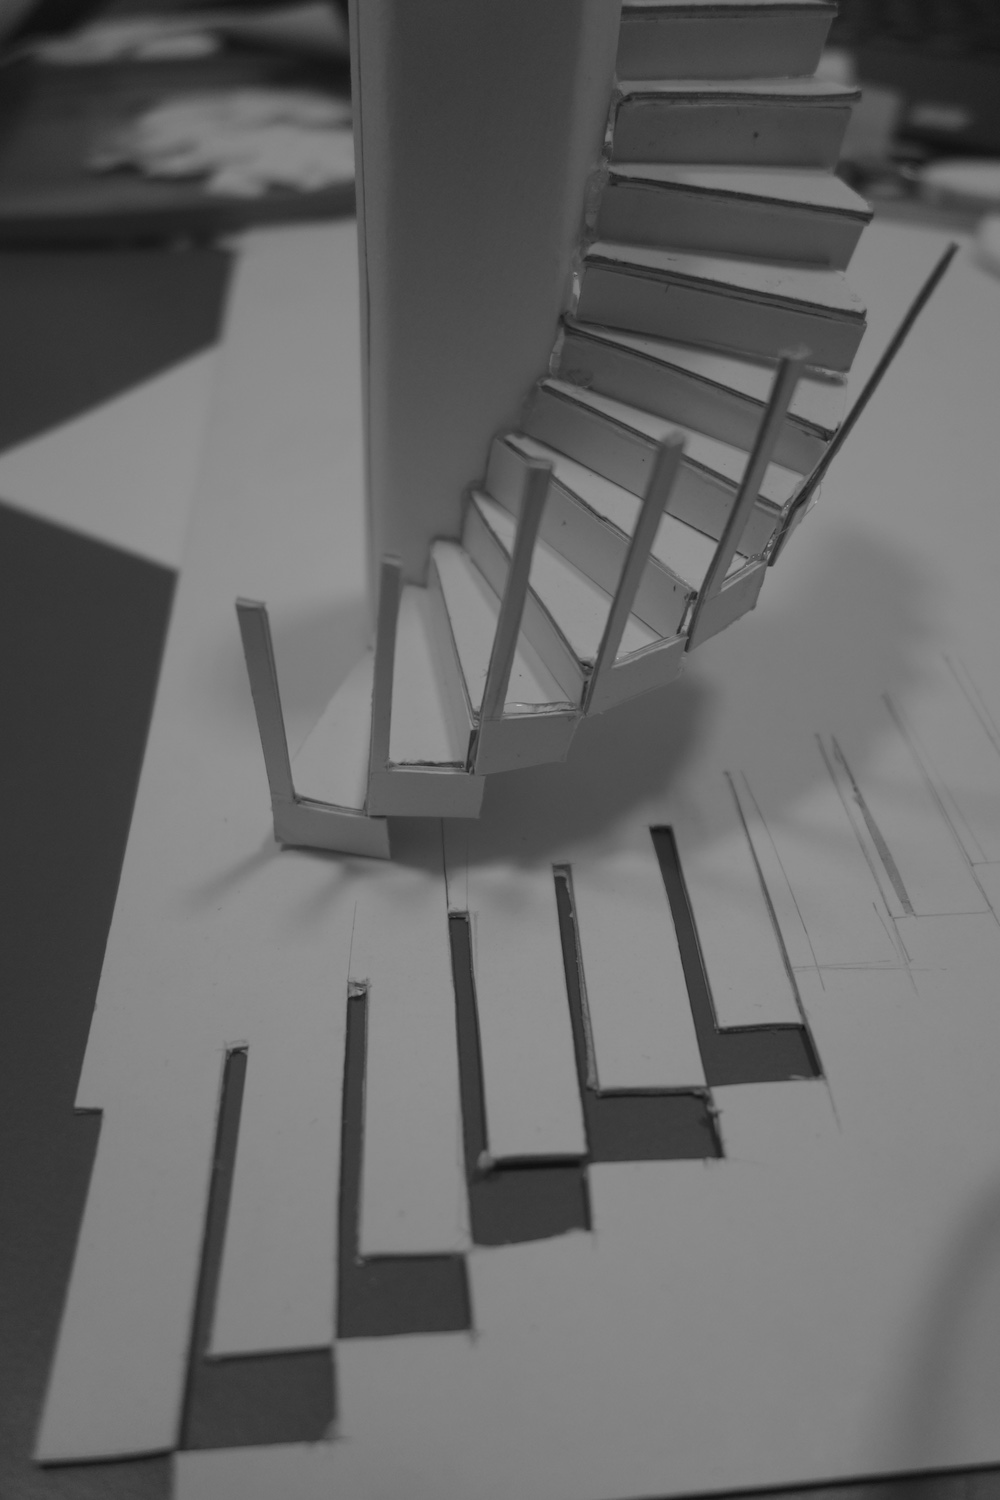
\includegraphics[height=0.13\textwidth]{steps7.jpg}
  \caption{Building the final spiral staircase design}
\end{figure}

One side of the top-floor would be the end of this staircase. The rest of it would be held together by the skeleton of the space. This was decided to be a hemispherical icosahedron.

\begin{figure}[h]
  \center
  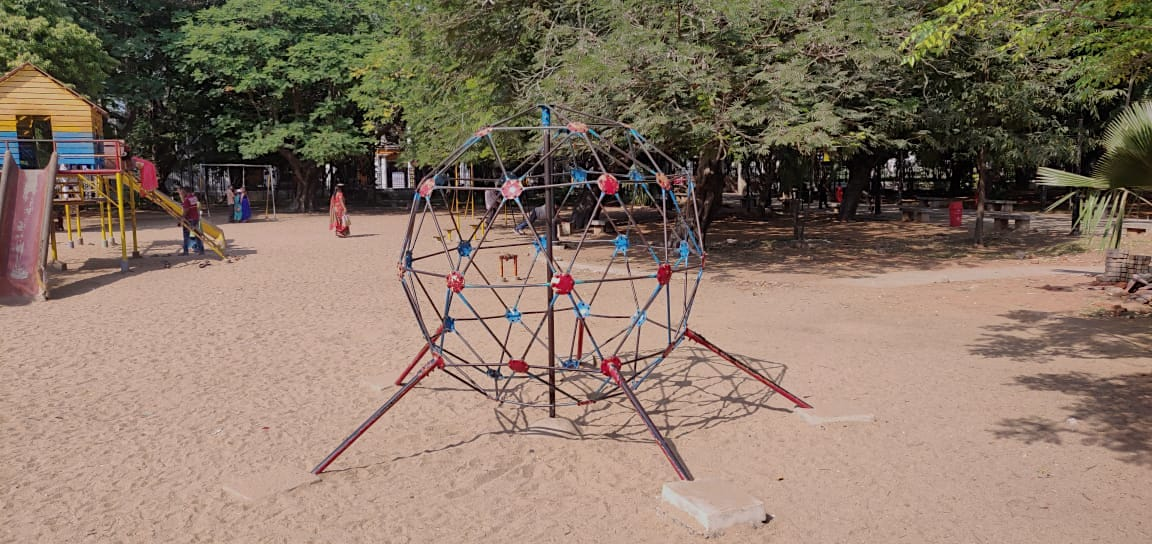
\includegraphics[width=0.5\textwidth]{park.jpg}
  \caption{Coincidental, yet insightful walk in the park. This icosahedron jungle gym helped gain clarity to construct the dome.}
\end{figure}

The decision of this form may be justified by the vastness one look of the sky has to offer. In the Hogwarts Great Hall, the real skyline is projected changing according to time. It would probably be nice for children feeling stuck/conflicted to stare into the sky and wonder, than into the wall. This fiction could be a reality, with on-button tinted glasses to make the room an enclosed space.

\subsubsection{Constructing the geometrical dome}
Assuming the unwrap from Blender would yield a reliable map of the proposed structure, a 1ft : 1cm scale print-out was cut and folded to build the following. 

\begin{figure}[h]
  \center
  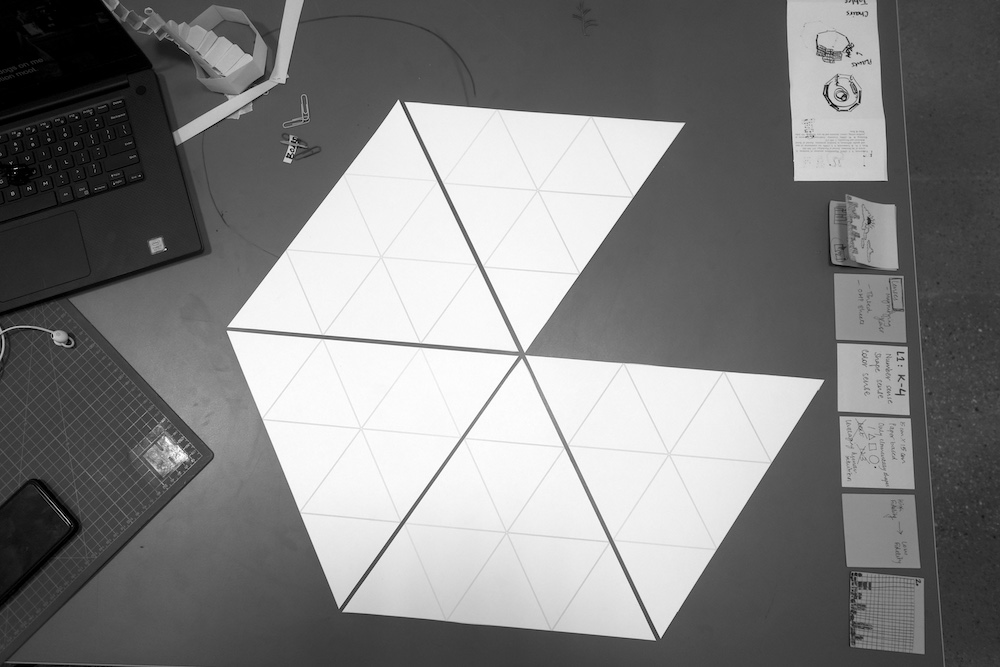
\includegraphics[height=0.21\textwidth]{dome4.jpg}
  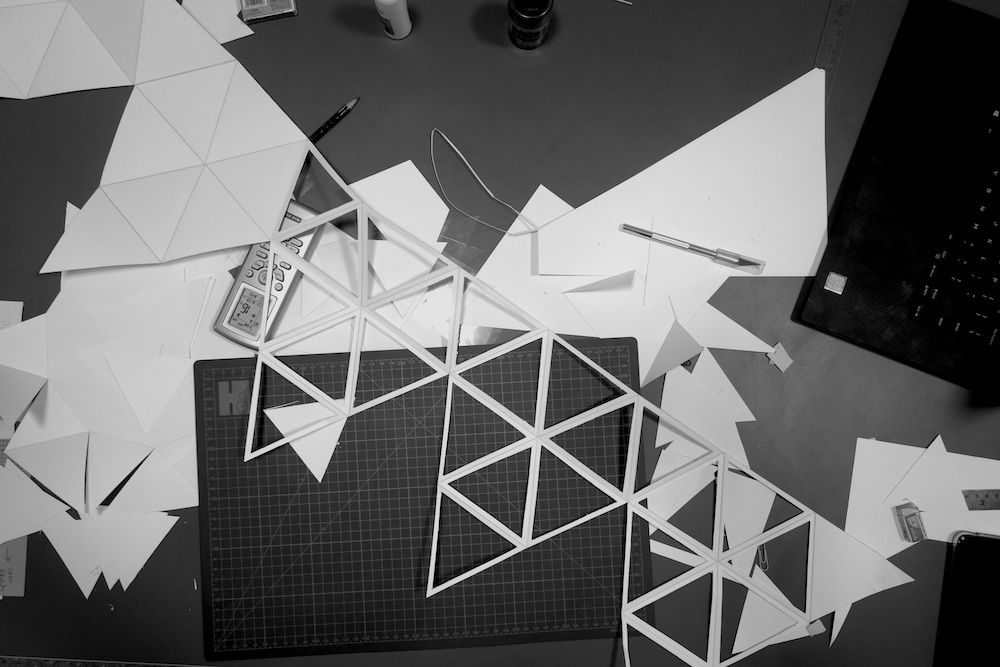
\includegraphics[height=0.21\textwidth]{dome5.jpg}
  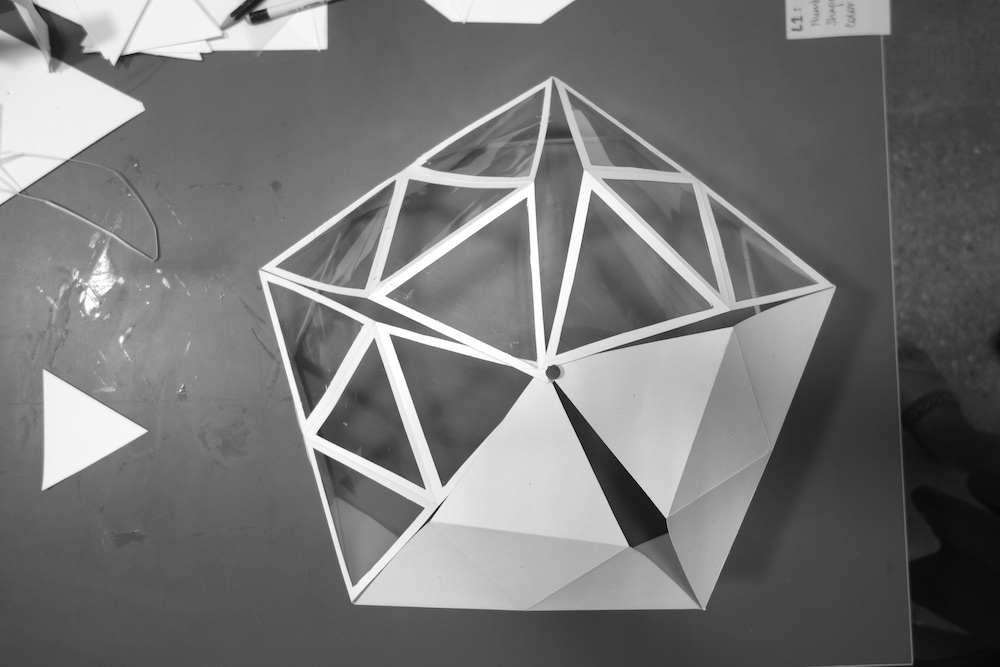
\includegraphics[height=0.21\textwidth]{dome6.jpg}
  \caption{The triangular sections were removed to be covered with OHP sheets for the window}
\end{figure}

The structure, seeming promising, lacked internal strength, that we felt was necessary to accommodate other objects. This was tackled by paper-taped toothpicks on every triangular edge. 

\begin{figure}[h]
  \center
  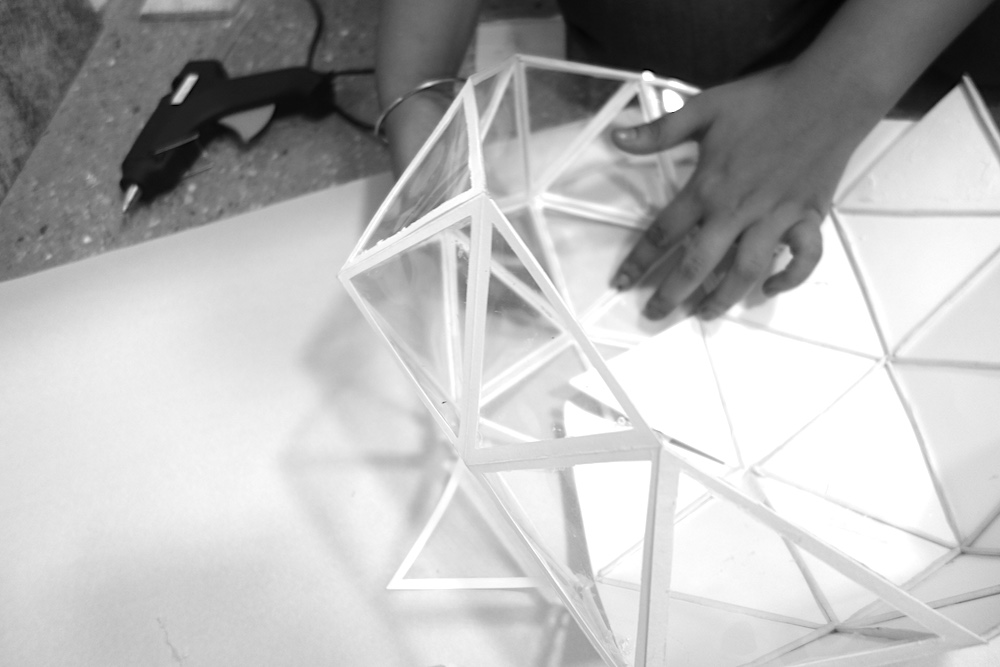
\includegraphics[height=0.2\textwidth]{dome7.jpg}
  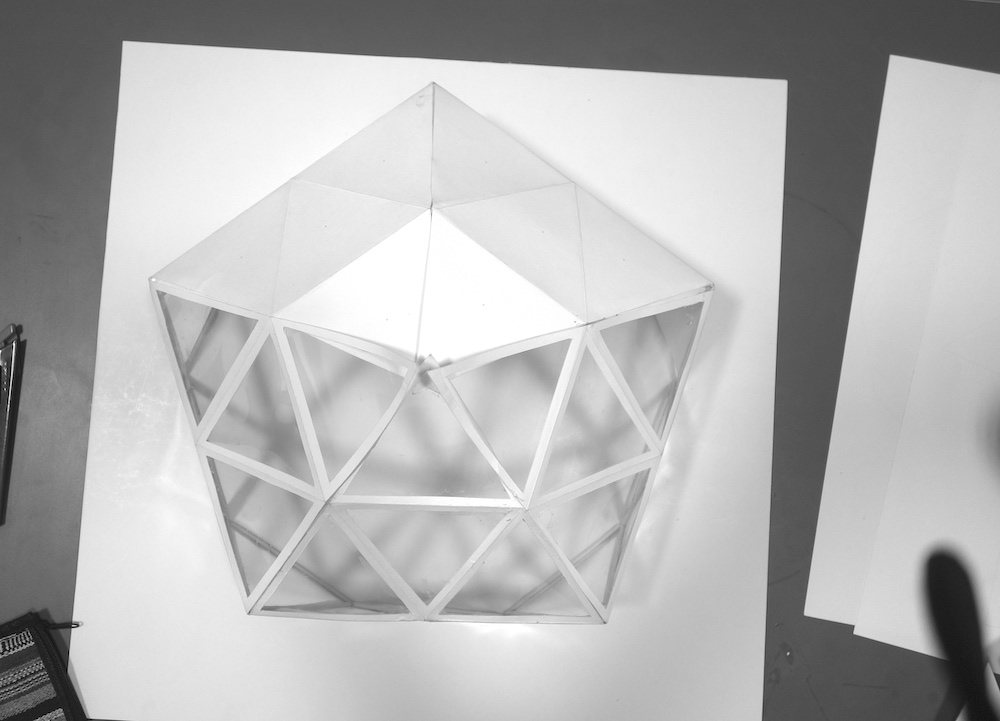
\includegraphics[height=0.2\textwidth]{dome8.jpg}
  \caption{The structure after toothpicks were placed to support the triangular panels}
\end{figure}

It was assumed that the toothpicks would bring rigidity to the structure. This was valid, except the form was being sacrificed by seeming to be flattened from the top. Icosahedrons have each vertex resting on an imaginary sphere. This form translated to a hemispherical ovoid. 

We further constructed 2 small-scale paper folded prototypes to cross-verify if our previous approach was faulty. Using both, edge to edge gluing and gluing with folded margins, the result was still the same.

A new, brick-by-brick approach was chosen next to accomplish the same form. This time, individual triangular pieces were cut to scale, and stuck together with glue gun at the specified angles. We began with constructing a pentagon first.  At the suggested angles, equilateral triangles failed to construct a pentagon. We devised a right angled triangle to help physically cross check the fitting between every triangle.

\begin{figure}[h]
  \center
  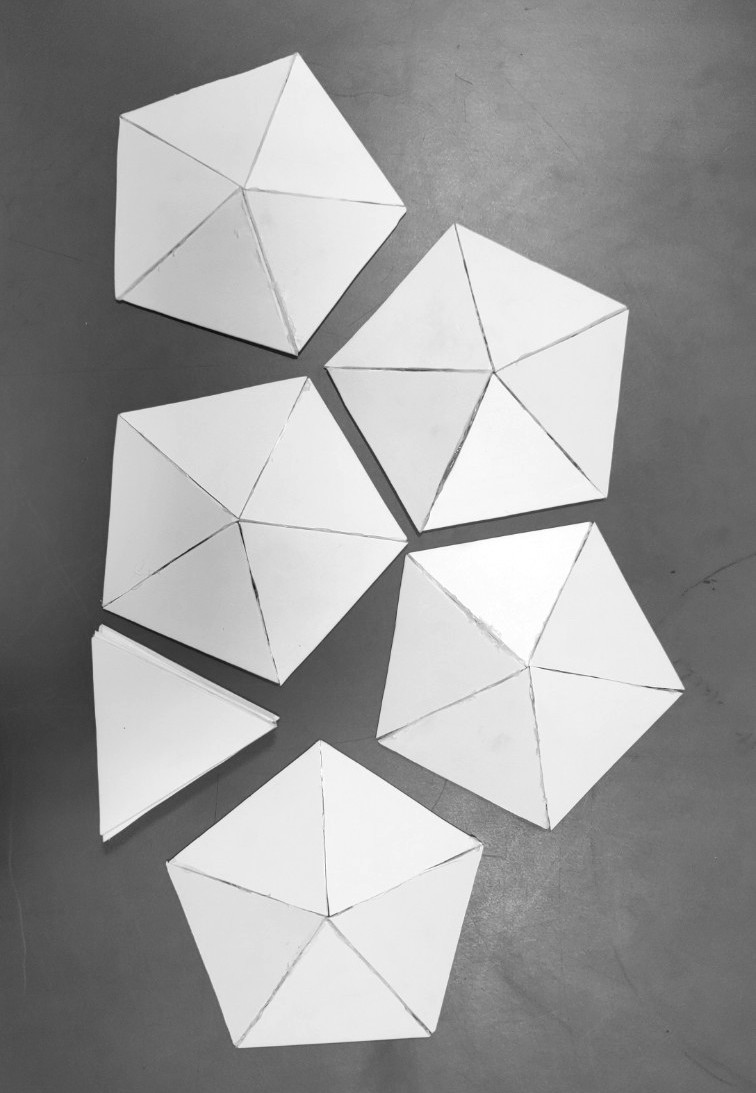
\includegraphics[height=0.3\textwidth]{dome9.jpg}
  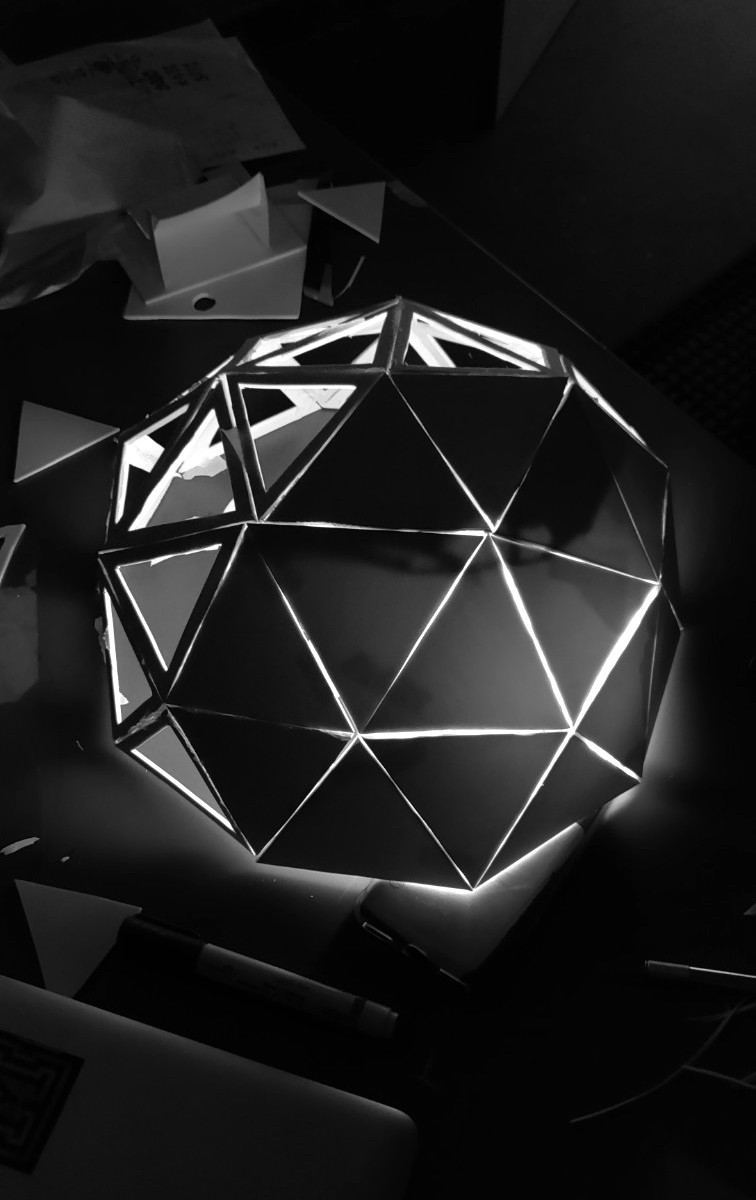
\includegraphics[height=0.3\textwidth]{dome10.jpg}
  \caption{Construction of the final dome}
\end{figure}

It was seen that every pentagon, constructed with isosceles triangles (10.9cm, 9.5cm, 9.5cm) could be joined together with an equilateral triangle (10.9cm,10.9cm,10.9cm) to accomplish our chosen form.

\begin{figure}[h]
  \center
  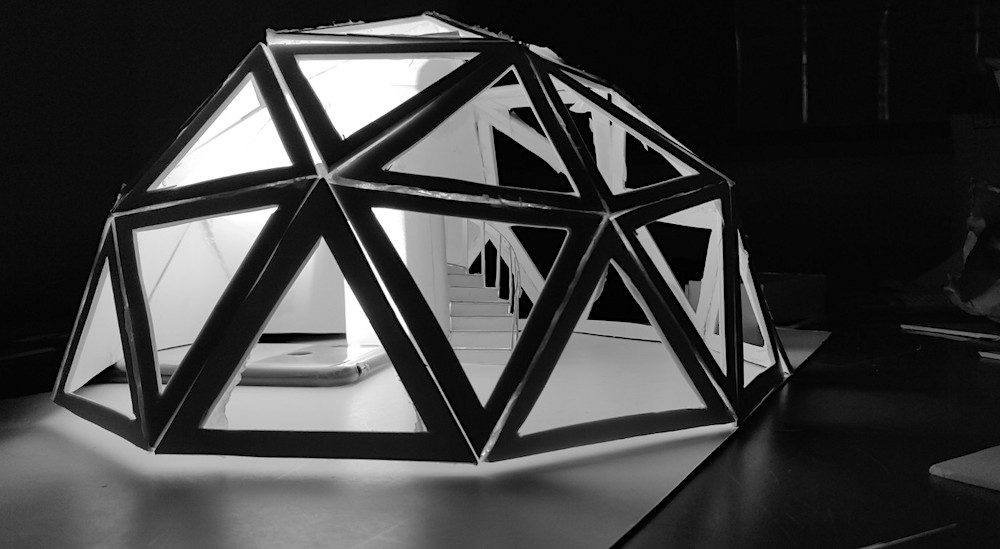
\includegraphics[width=0.6\textwidth]{dome11.jpg}
  \caption{Discoverdrome - with lighting from inside}
\end{figure}

\subsection{Furniture}
The key motivation behind all furniture was modularity and easy accessibility in the space. This meant choosing forms that would make good, dynamic puzzle pieces. Maintaining the same geometric theme, tables were given hexagonal forms, with the choice of sharing with another facilitated by a middle screen to barricade space. 

\begin{figure}[h]
  \center
  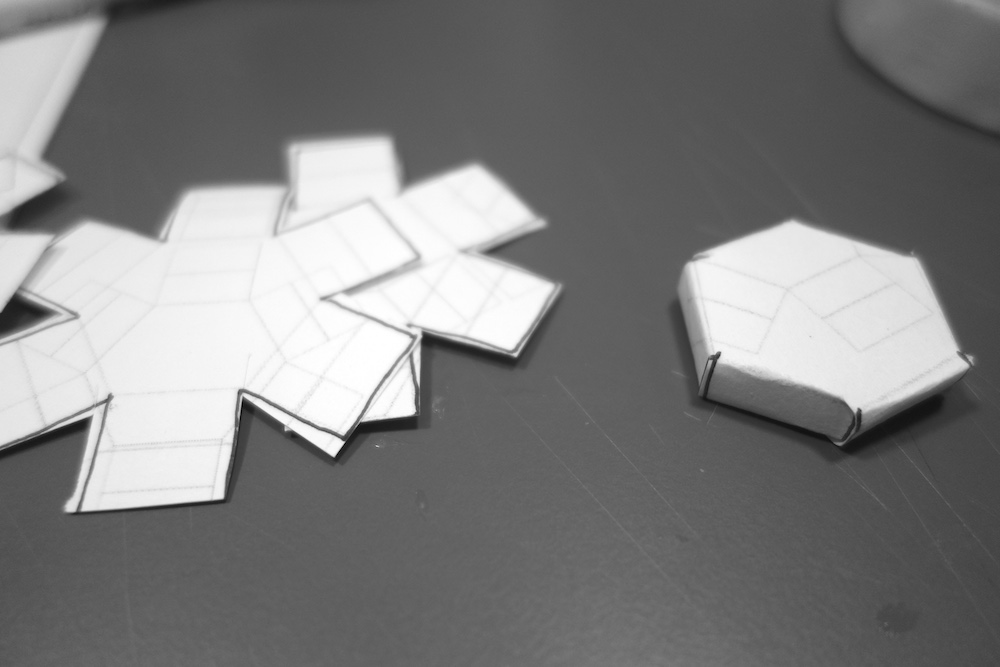
\includegraphics[height=0.15\textwidth]{furniture1.jpg}
  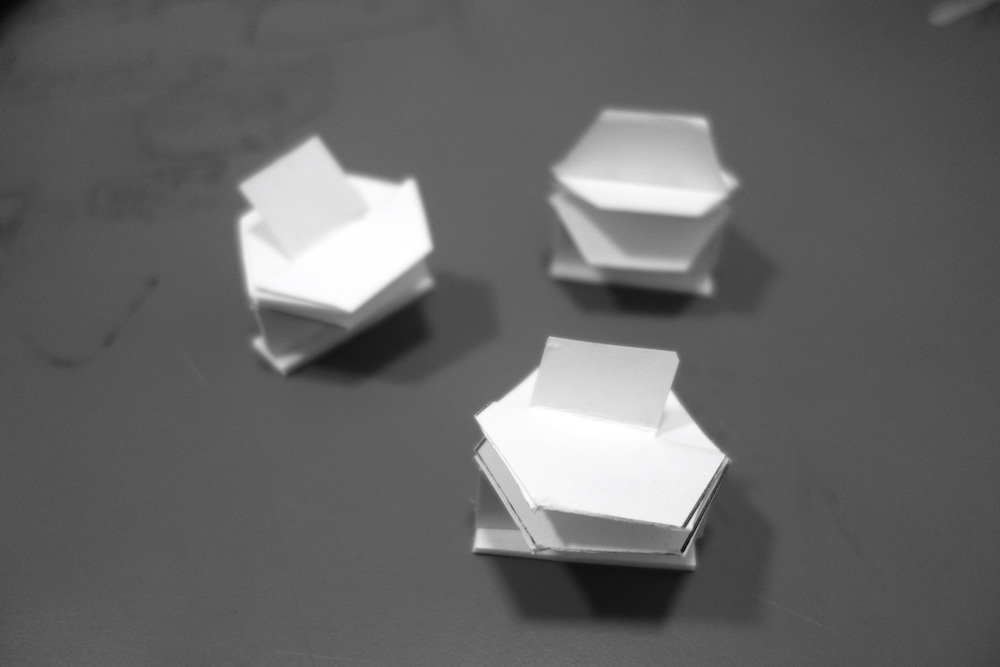
\includegraphics[height=0.15\textwidth]{furniture2.jpg}
  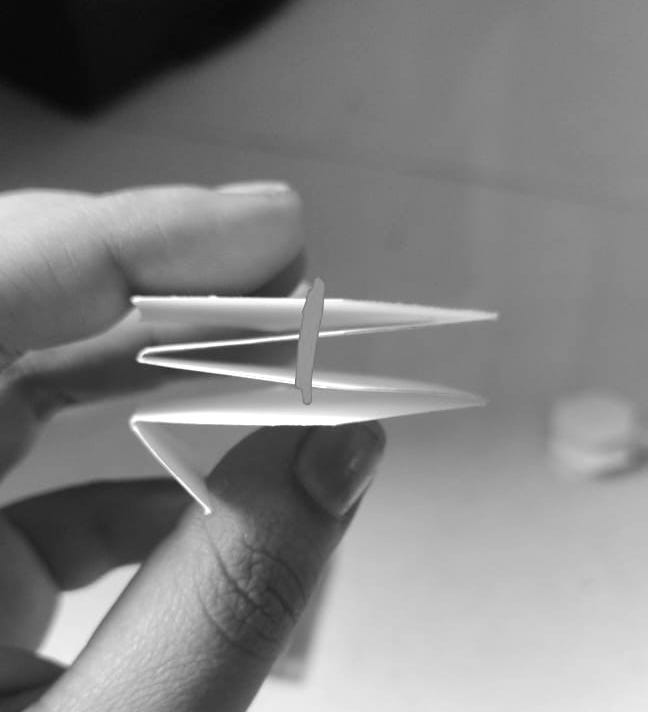
\includegraphics[height=0.15\textwidth]{furniture3.jpg}
  \caption{Tables -- earlier just hexagonal blocks, folded for accessible shelves and storage}
\end{figure}

The seating was decided to be movable, comfortable and easily-accessible. Varied softness cushions, as well as rectangular blocks were built to suit the space.

\begin{figure}[h]
  \center
  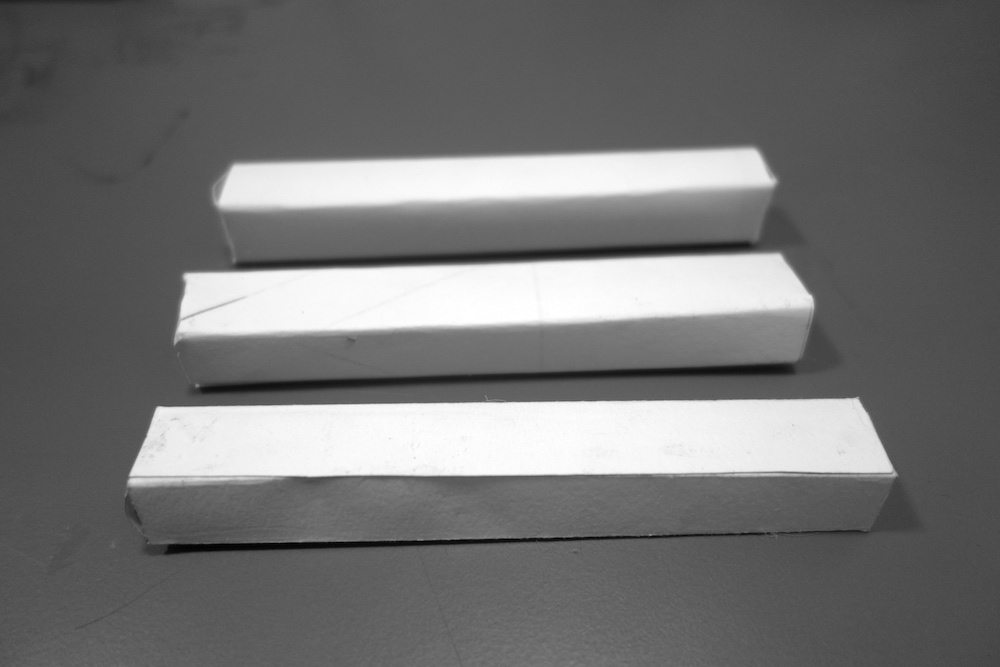
\includegraphics[height=0.15\textwidth]{furniture4.jpg}
  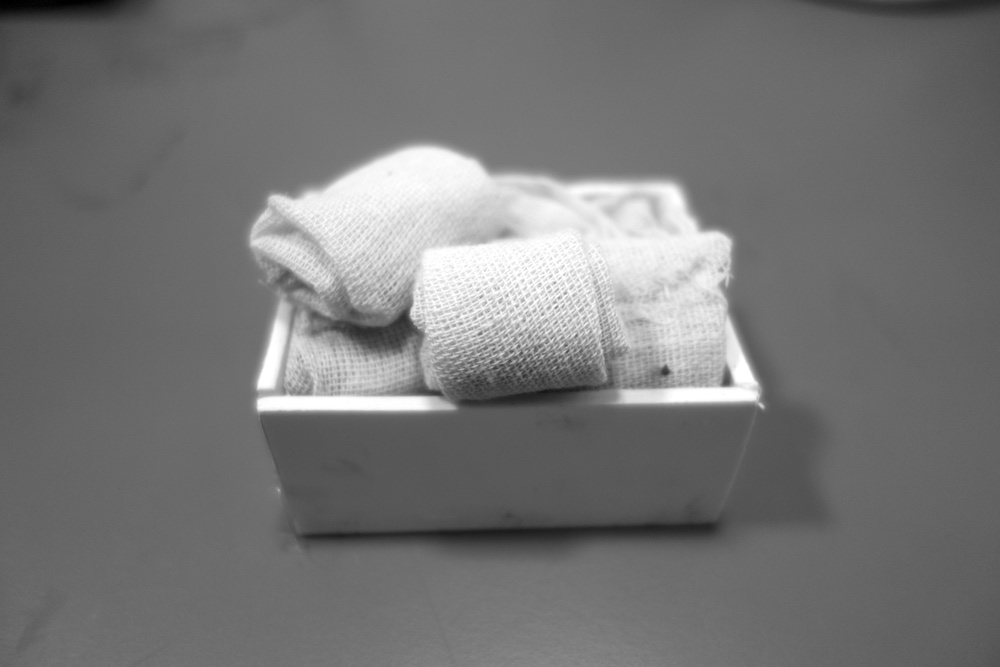
\includegraphics[height=0.15\textwidth]{furniture5.jpg}
  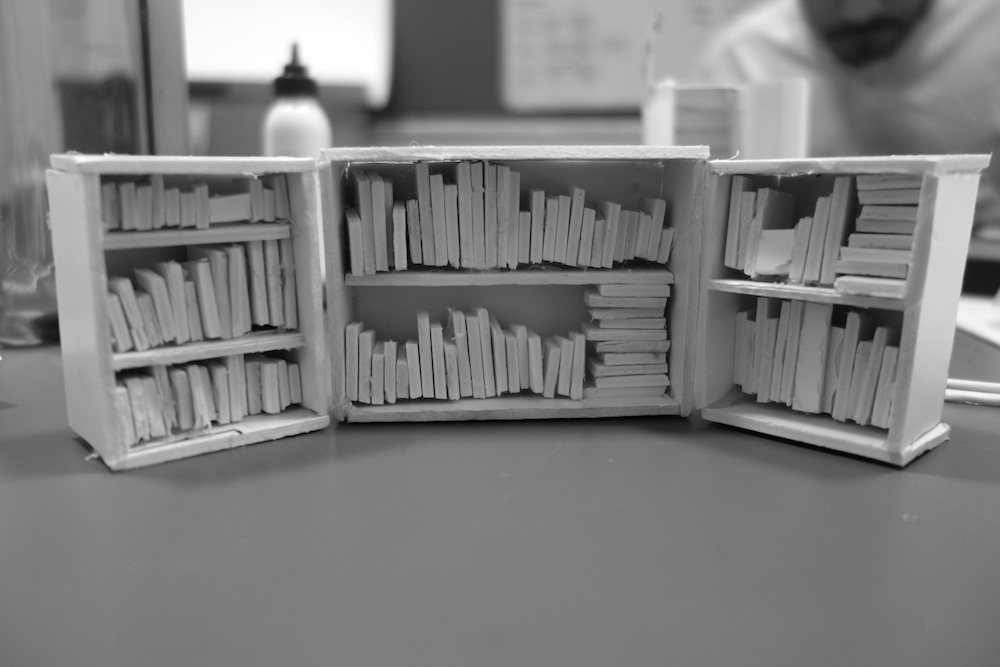
\includegraphics[height=0.15\textwidth]{furniture6.jpg}
  \caption{Seating and bookshelves for the library}
\end{figure}

As objects increased in making, the idea seemed real. In a literal sense, the future began to look physical. A constant switch between speculation and making makes room for experimentation while playing with constraints, instead of worrying/planning about them.

\begin{figure}[h]
  \center
  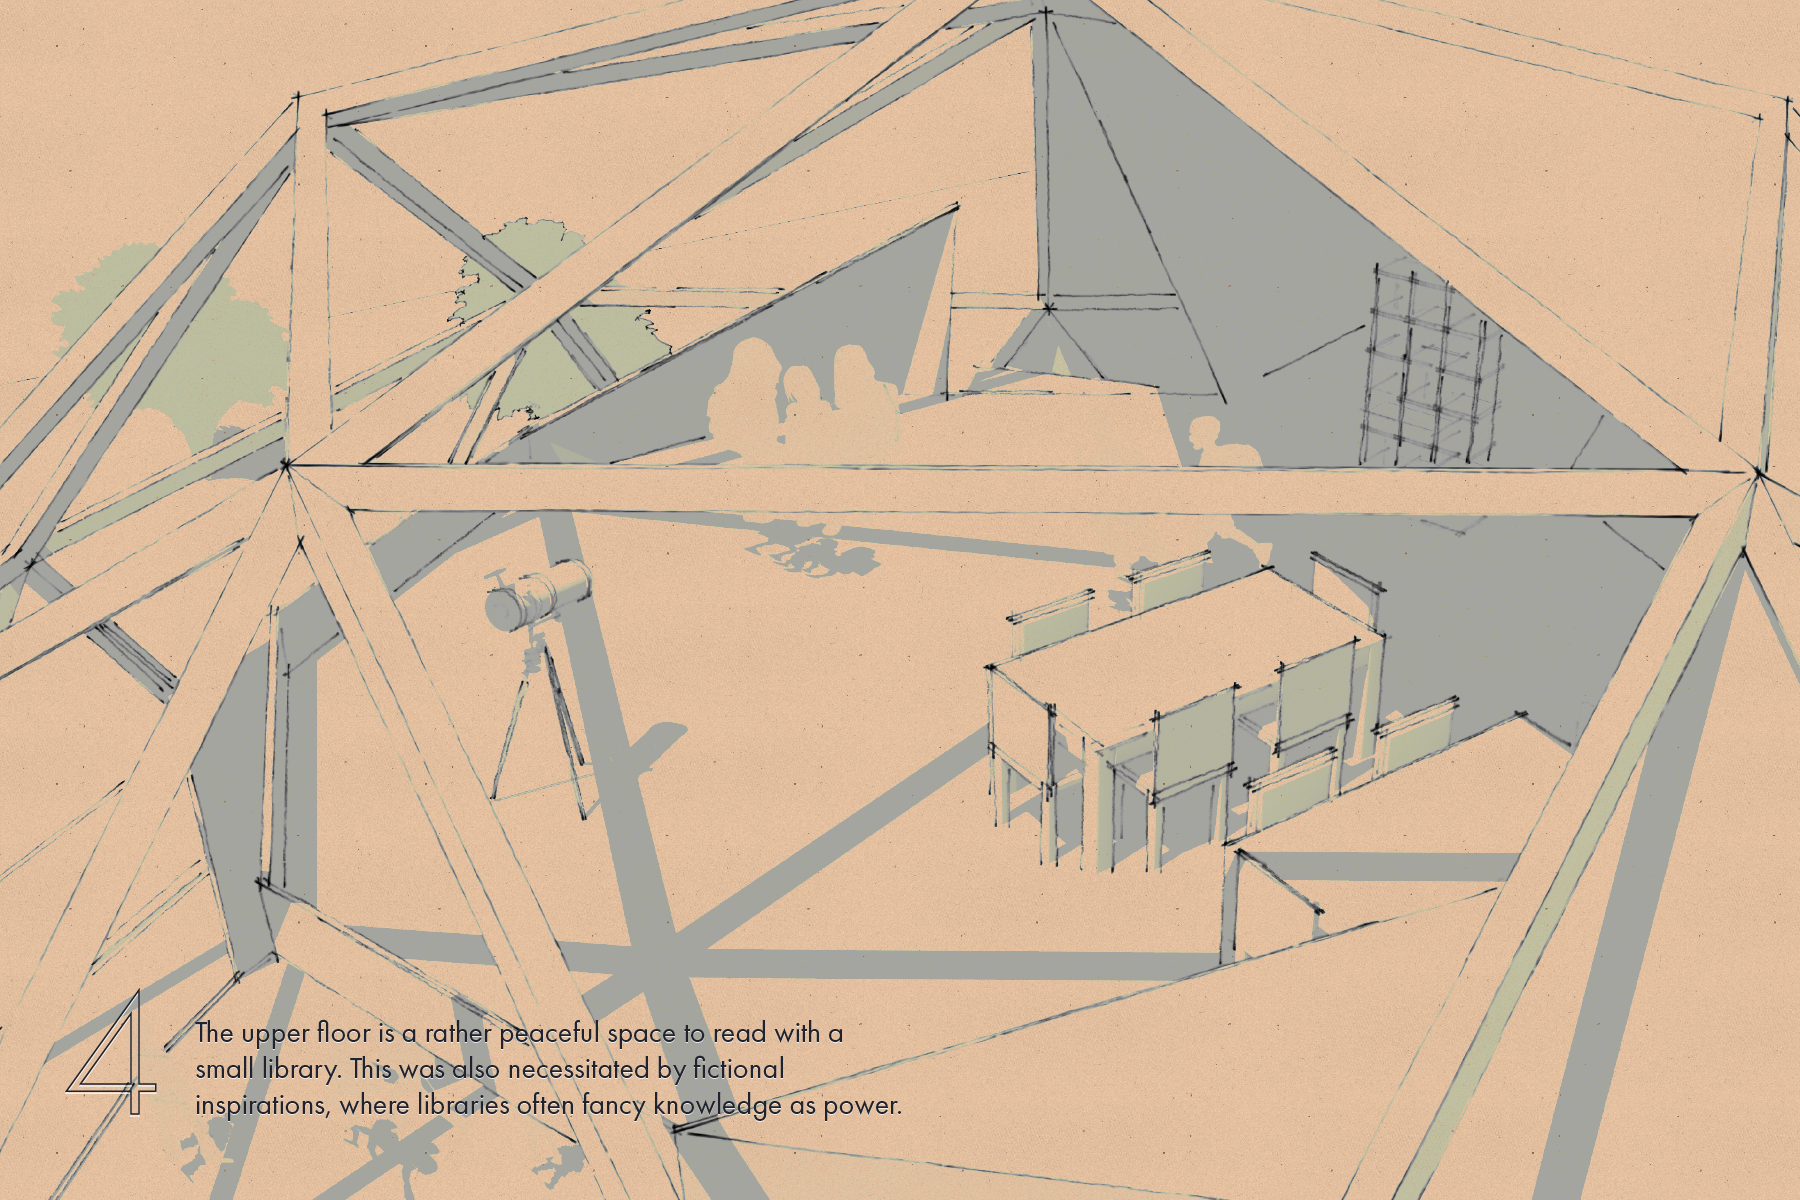
\includegraphics[width=0.9\textwidth]{discoverdrome_4.png}
\end{figure}

\section{The Letter}

Dear Earthlings of the future,

Our current education system dejects me. Don’t get me wrong; I grew into the person I am and learned how to think because of it. But back in my day, tussles to collaborate were regular. Not everyone liked the theory, not everyone enjoyed practicals, because they would all be expected/wish to master everything. Not everyone would agree the experience was joyous. The collaboration wasn't dead; people only needed the easy ability to understand related fields better. All counter-initiatives to improve would get lost in the system and the path to knowledge would only lead to an individualistic workflow. Marks and grades would rule the fate of the knowledge one consumes. Schools (are) were majorly utilised as temples of information suited to a few who could master its safekeeping. That made dealing with application of this knowledge system 2, a little devoid of smart-hacks that could be useful in the learning experience. What good is this approach if the space doesn’t benefit all?

\begin{figure}[h]
  \center
  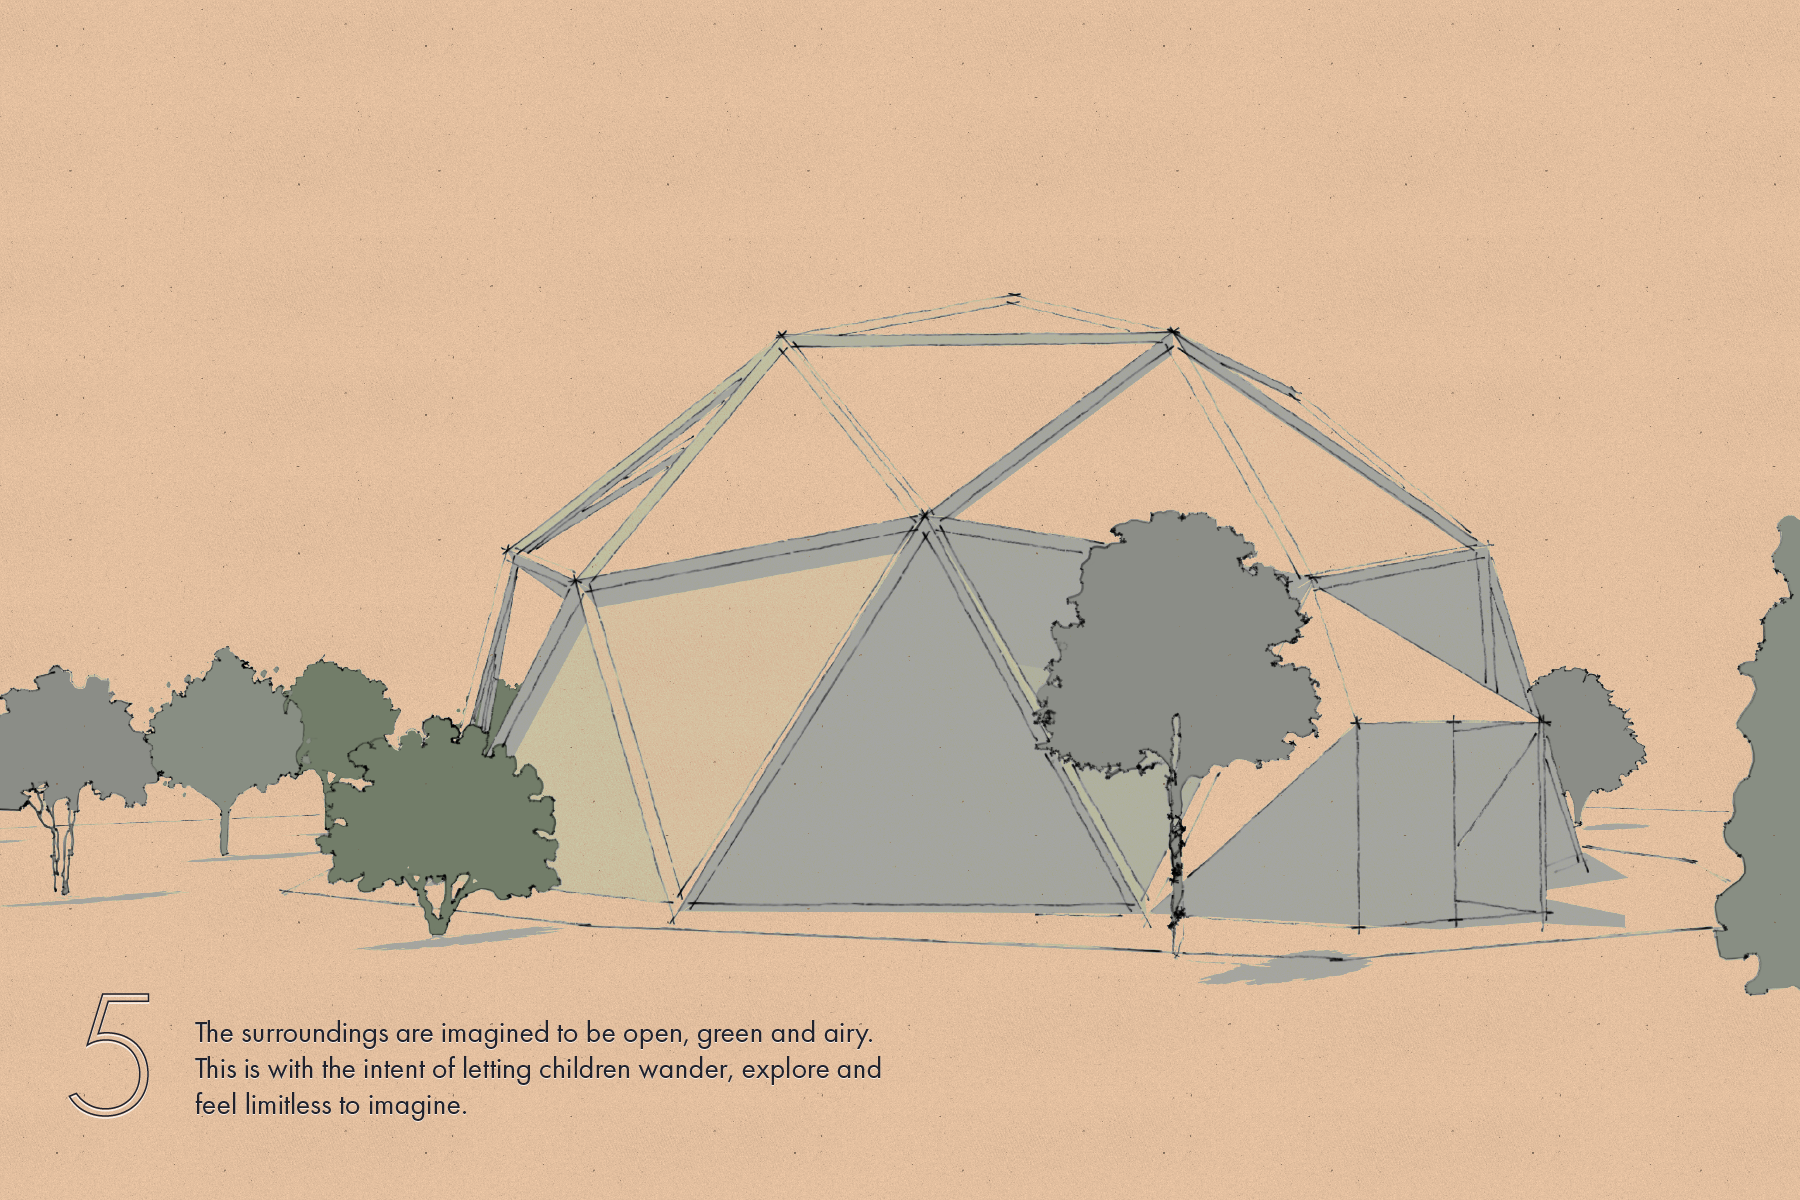
\includegraphics[width=0.9\textwidth]{discoverdrome_5.png}
\end{figure}

Rapid growth in technology requires individuals to be aware, active and pivotal in writing this fast-developing history. One way of accomplishing this is catering for the experiences that resonate and travel with children in their paths to knowledge. This means, teaching them both the knowledge and real-world application in ways that they retain easily. Currently met by the classroom-blackboard approach, we expect the future classroom to retain this sustained methodology as well as accommodate new, open ended interactions in the same space. The right understanding of fundamental concepts needs a firm foundation that should be found in the classroom itself. The comfort of expressing oneself in a large group can also be gained from the space.  

When I was in school, my classroom had cuboidal tables and pillars we would hide behind. Most of the overall space would be occupied by cupboards, tables, chairs and the blackboard making it a rigid space to experiment in. I would share my table with my partner, and most of the interactions in class would be sitting in the same spot taking notes and building on ideas. Even though this system was successful at our time, we can imagine ideas we developed later could have made sense to us earlier, had we been exposed to a few interventions earlier.

Deciding every aspect of the classroom, from accomodation size to what and how much of the furniture everybody gets to use, we kept in mind that we expect  kids from different backgrounds, careers and beliefs coming together to do good for humanity some day. The space should be able to accommodate room for their conflicts to resolve. This would mean providing all possible ways of reshuffling the space. The tables and chairs were given hexagonal and easy to use forms to provide a dynamic workspace. The chairs, as movable floor cushions also imply the same idea. The floor is a huge polygonal area that can be divided easily for personal workspaces. We even imagined a little Harry Potter feel through the emphasis on still having books around, possibly floating in the space approached through a royal staircase, welcoming you to pursue your intellectual inclinations.

Positive energy is reflective of clarity in thought and organisational workflow. With minimal hindrances causing from space emerges good design to suit the growth and sustenance of this energy. To acknowledge that ideas apply everywhere and should be free to grow and be heard isn’t an ingenious breakthrough. However, getting them to suit the current needs of the world is important. Problem solvers of the future will face the complex problems of their time, which may never have been encountered before. What if their team on board was too shy to be honest about their opinions? What if they pushed back some really phenomenal ideas for the lack of definite understanding or willingness to explore?

\begin{figure}[h]
  \center
  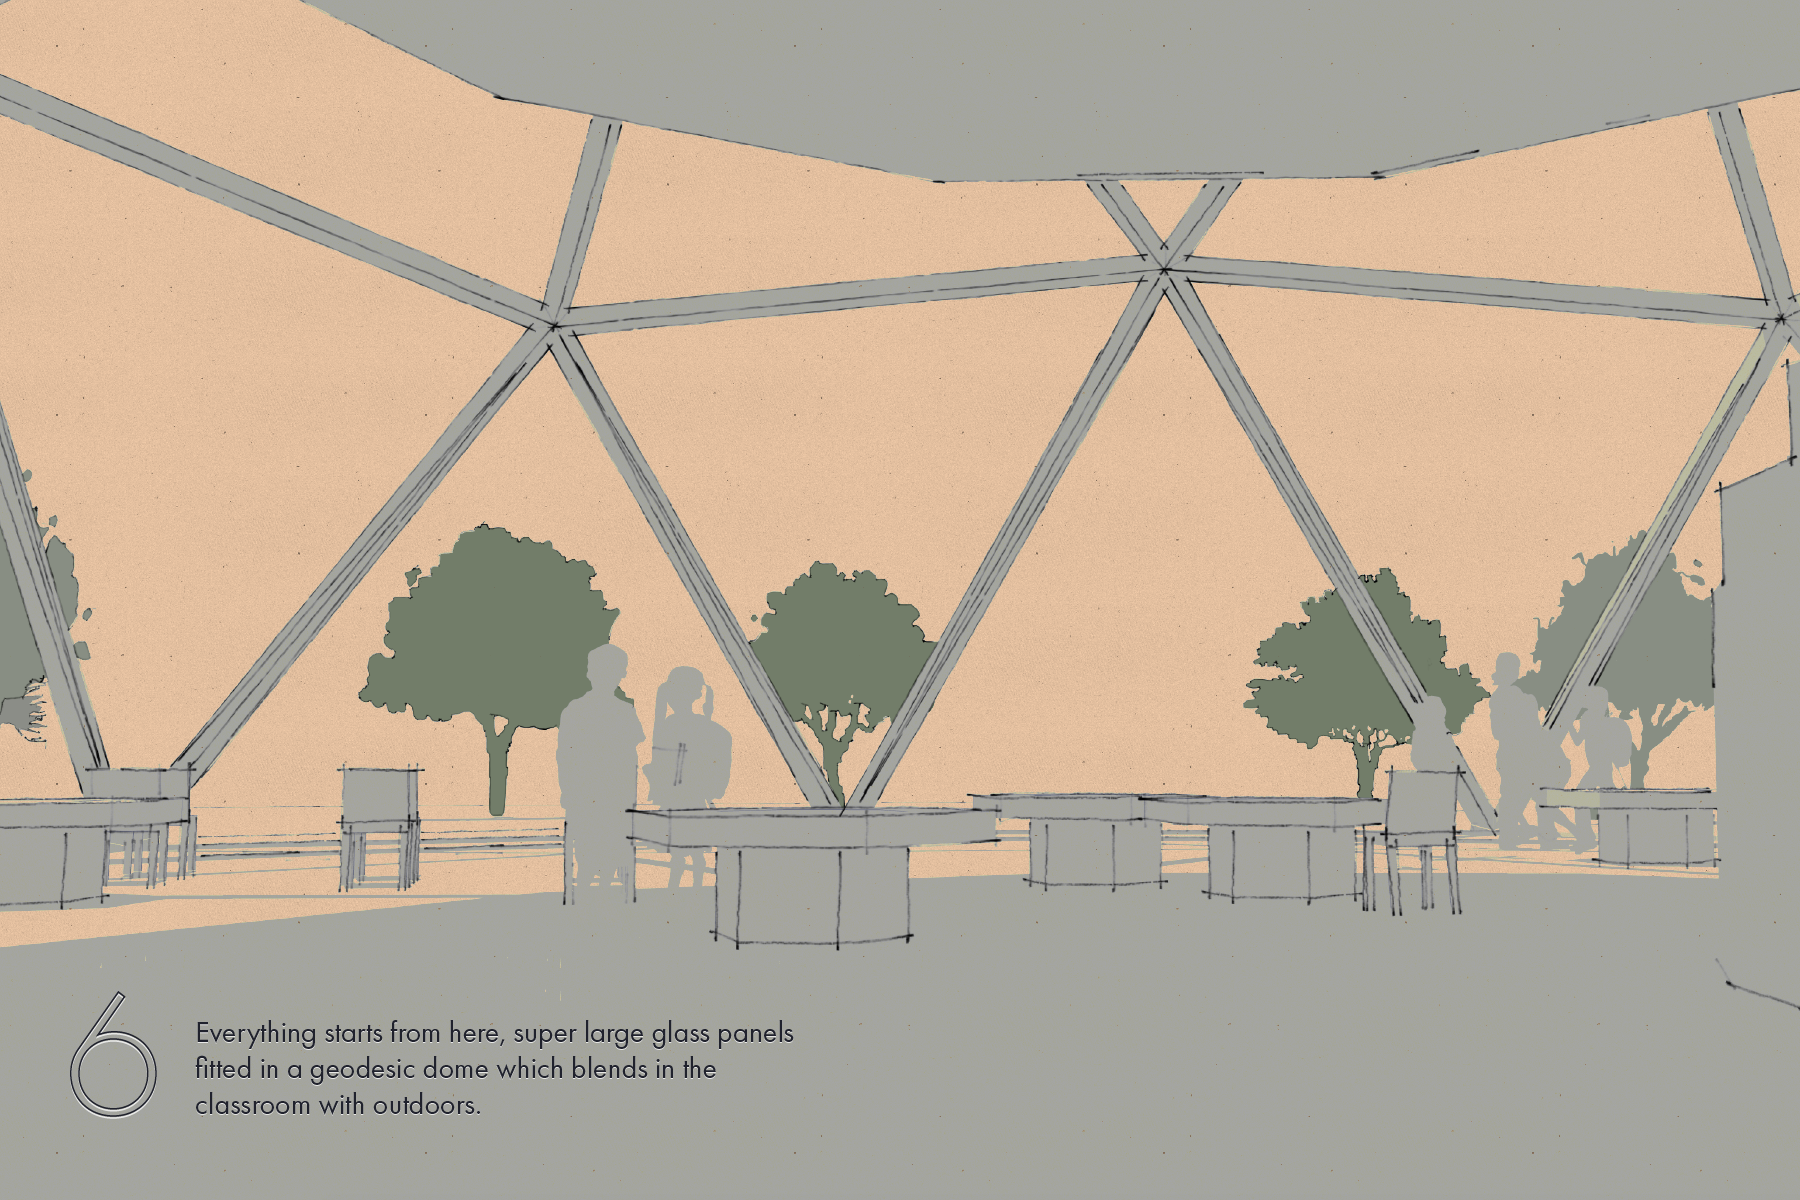
\includegraphics[width=0.9\textwidth]{discoverdrome_6.png}
\end{figure}

If they got over these common but strong factors in workflow, their goals can be met faster, don’t you think? Their approaches should not be limited by communication or exploration fallouts. Educational standards should be in sync with the progression of the world. 

I hope this letter reaches you in good faith. The model, where I hope you found this letter in, retains the mark of the maker. Capt Mashes and I, from Earth C-137 imagined what the ideal classroom would look like, in a sustainable, far-away future..

Explore. Imagine. Emerge!

Signing off

Simran Singh

Human-Centered Designer (by 2020)

\ang{13}06'15.4''N, \ang{77}34'21.1''E \hspace{0.2cm} 11.07.2019 \hspace{0.2cm} 23:30

\begin{figure}[h]
  \center
  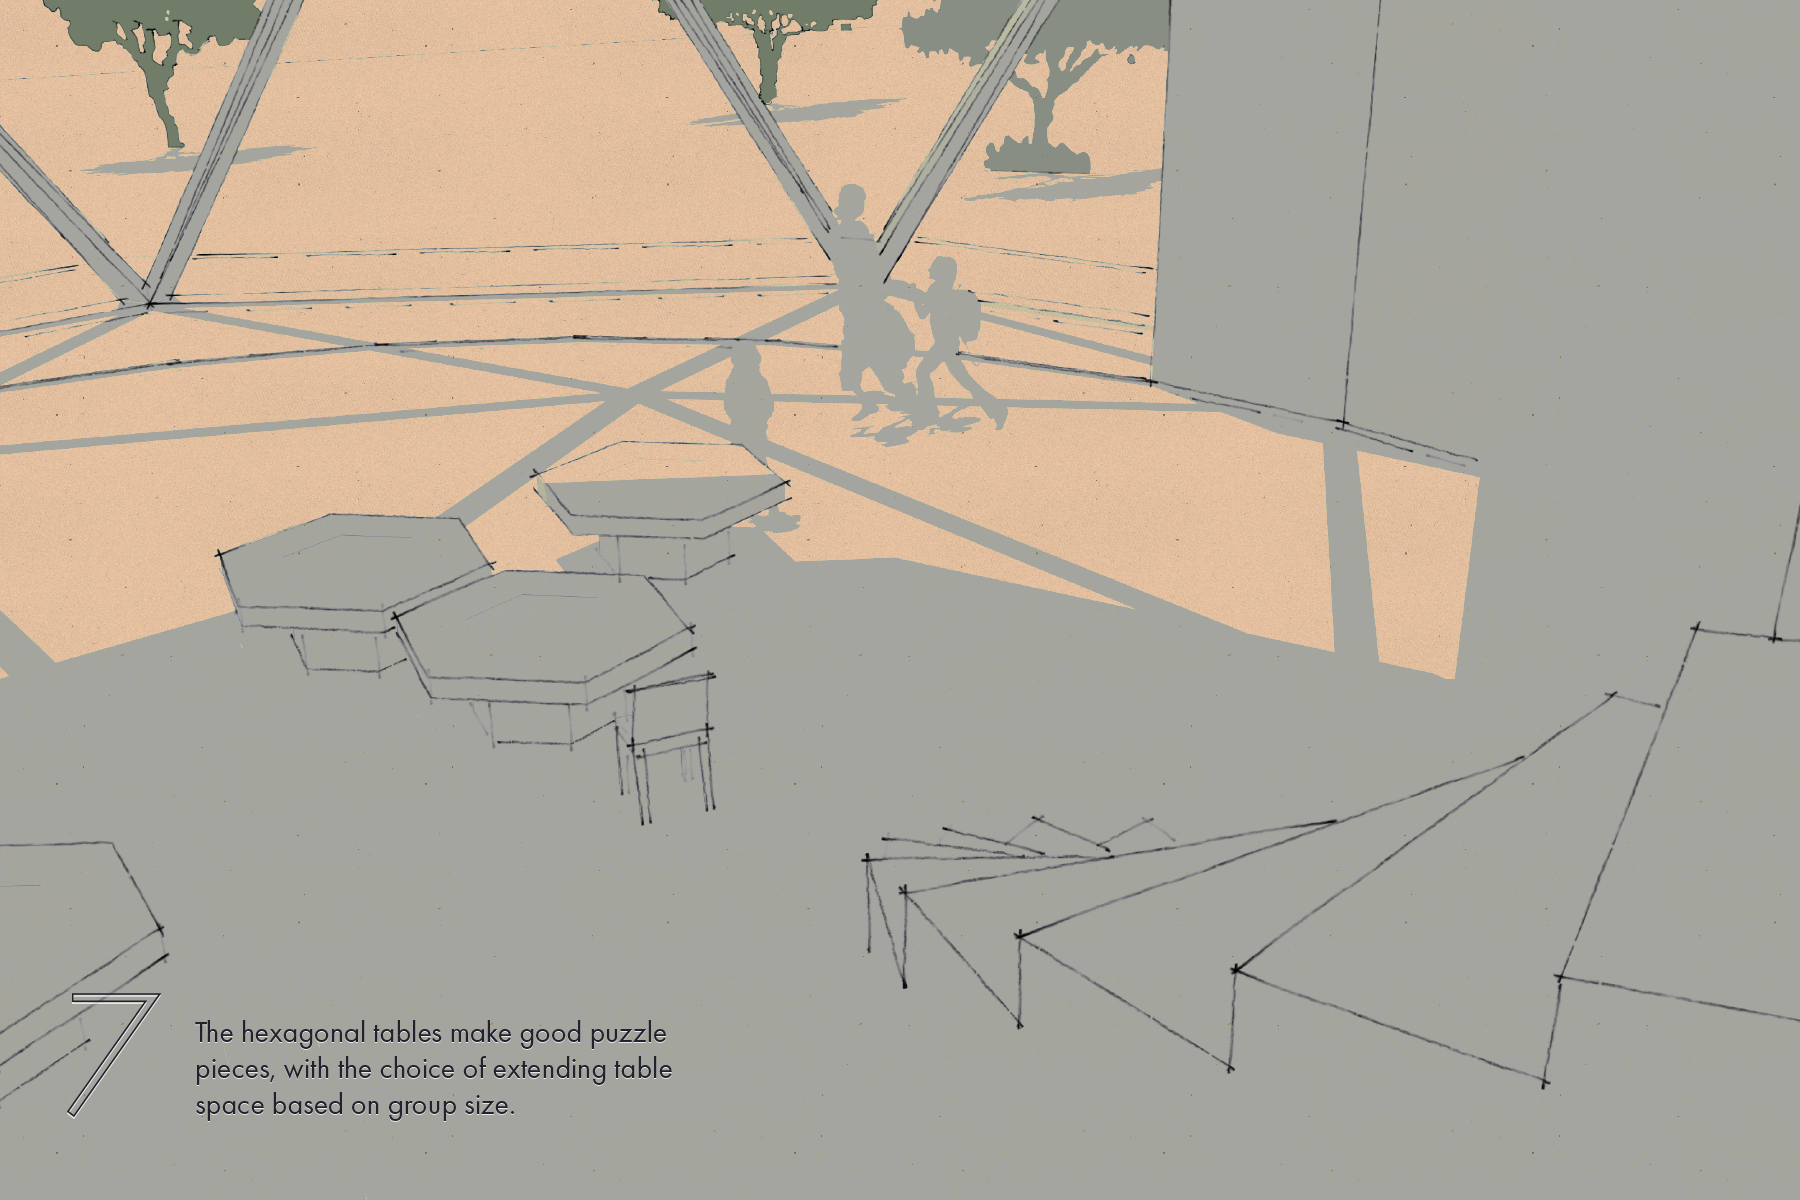
\includegraphics[width=0.9\textwidth]{discoverdrome_7.png}
\end{figure}


\section{Reflection}
Plans and blueprints hold responsibility of imparting a certain experience on implementation. Each little decision shapes the way it would emerge. Intended to be a short-lived expedition, this project offered to imagine a futuristic view of the kind of school we would have liked as children, enabling us to assume the extents of the growth in technology by the year 2100. The classroom of the future will raise the people of the future, people who are smart, active and able to break complex operations into minute details to intervene. The classroom built here is a space for such individuals in their years of schooling with elements that resonate with our current ideas for the future.
 
We see the world emerge with better technology and design solutions, enabled by successful learners and creators of our time. But what about those great ideas that are restricted by our own limited ideologies of learning? 

\textit{“Students not used to prolonged thinking on a single problem start off well. However, soon they find motivation and inspiration leaving them, and they start dreading working on the problem as failure would lead them to question something they (by now) crucially identify with: “smartness”. Procrastination kicks in, and soon the student is busy in a diverse set of academic (but non-research!) activities to hide the reality of not working, like writing complicated scripts to automate their soon-to-be-coming publication phase, optimizing their daily vitamin B12 intake, getting heavily involved with political and religious movements and so on. Few students are able to critically introspect, which is reasonable since society has informed them that smartness is what matters, and if they are unable to solve the problem quickly, the logical conclusion is that they are not smart.” -- Nabil H. Mustafa, On Being Smart}

Understanding, realising and living these limitations in the present, we see the fallbacks of lack of concentration and affected productivity each day. Learning from our own extended experiences in and because of our school classroom space, the giveaway for the future here is a set of ideas, emerging into a process holding plausible interventions we feel are imperative. 

The plan was led by an iteration on-the-go approach. This meant constructing the idea instead of talking about it, and building onto this physical artefact to realise what we imagine. In this way, with every added object comes a conscious cross-check of whether the idea is translated through the space. For example, it is seen that children often have low attention spans. For a good use of their own time in their learning years, their minds should be kindled with curiosity. This is generally enabled by the objects in the space and the space itself, since the user would walk up to it and interact with it instead of an imposed action. A problem of this kind requires funding and time to implement universally; constraints that hinder the actualisation of an important design solution. However, placing it in the future, next to logical and conceivable concepts can actually enable us to set the dominoes in motion. We saw this happen when the building structure of our choice took multiple iterations, brainstorming sessions and approaches to understand how it may be constructed correctly. We probably wouldn’t even think there would be a problem in construction, if we didn’t try to create the structure ourselves first. We may have been able to read in theory what problems may arise, but we wouldn’t thoroughly understand them without perceiving it together and physically.

Similar was the case when we started to think, how the space may be made better functional and flexible. Every team requires their own kind of execution. This would mean free movement in the space and objects acting like lego pieces: setting ground for the emerging theme of modularity. The thought of easy access to resources in the space made us think of integrating a library in the same space. Collaboration requires every individual to understand, interpret, create and share their ideas; enabled by a sense of comfort in the space. This comfort can be provided discreetly by simply placing objects and no restrictions for them to suit themselves best. 

We understand that the future brings with itself its new complications, and we speculate that the need of then hour would be effective solutions relying on productive, sharp and quick minds that steer the way ahead. This can be met by enabling everyone to find their choice of learning style and letting them cultivate and emerge from it. Our own classrooms were not given much thought, seem outdated, or varied differently for the number of people who lack curiosity or interest. If this project were to really be implemented as the intended classroom, it would be remarkable to see the work of these spatial interventions shaping better, smarter humans of the future.

\vspace{1cm}
\footnotesize \textbf{Acknowledgement.} I would use this space to thank the following people, who kept reminding me from time to time what a beautiful process making is. Karan Dudeja, for helping us construct, de-and-re-construct the icosahedron to its current form. Gunika Sahni, Anamika Samanta and Sabareesh Nair, for making me take breaks just before I would exhaust myself using the paper-cutter, patiently accompanying my work and occasionally cutting some paper themselves. Blender, for making this project less laborious. I know a hundred different ways I would have deviated working with building blocks. And Gaurav Singh, for mentoring me through the entire process, and weaving my learning experience towards an ever-evolving unfolding journey. Discoverdrome is appropriately named.

\vspace{0.5cm}
\textbf{About the author.} Simran Singh is a Human-Centered Design student pursuing her undergraduate degree at Srishti, Bangalore. An analytical-dreamer, her work focuses on understanding the use-cases of emerging technologies and applying it in a user-friendly context. She sees value in algorithmic thinking to help understand, decode and apply at the design context.

\vspace*{\fill}
\rule{\textwidth}{0.4pt}
\footnotesize \mscpy. All rights reserved. This paper or any portion thereof may not be reproduced or used in any manner whatsoever without the express written permission of Mathscapes and the author(s) of this paper except for the use of brief quotations in a review.

\end{document}
